\documentclass[11pt,letterpaper]{article}
\usepackage{graphicx}
\usepackage{cite}
\usepackage{url}
\usepackage{amsmath}
\usepackage{amssymb}
\usepackage{color}

\include{basic-macros}

\setlength{\textheight}{9in}
\setlength{\topmargin}{0in}
\setlength{\headheight}{0in}
\setlength{\headsep}{0in}
\setlength{\textwidth}{6.5in}
\setlength{\oddsidemargin}{0in}

\newcommand{\equationsize}{\small}
\newcommand{\bibliographysize}{\small}
\newcommand{\captionsize}{\small}
\newcommand{\captionspace}{\vspace*{-0.2in}}
\newcommand{\afterfigspace}{\vspace*{-0.2in}}

\newcommand{\Section}[1]{\vspace*{-0.08in}\section{#1}\vspace*{-0.08in}}
\newcommand{\SubSection}[1]{\vspace*{-0.08in}\subsection{#1}\vspace*{-0.08in}}
\newcommand{\SubSubSection}[1]{\vspace*{-0.08in}\subsubsection{#1}\vspace*{-0.08in}}

% set spacing in figure caption
\newcommand{\figurespacing}{\renewcommand{\baselinestretch}{1.0}}

% symbol footnote: use \symbolfootnote[#]{footnote} to invoke with
%    1 = *; 2 = dagger; 3 = double-dagger; 4--9 = see latex docs
\long\def\symbolfootnote[#1]#2{\begingroup%
\def\thefootnote{\fnsymbol{footnote}}\footnote[#1]{#2}\endgroup}

% bold paragraph headers
\newcommand{\boldstart}[1]{\vspace{0.07in}\noindent{\bf #1}}

\newcommand{\comment}[1]{}
\newcommand{\todo}[1]{{\textcolor{red}{\bf [#1]}}}

% math shortcuts -- from Todd
\newcommand{\vx}{{\bf x}}
\newcommand{\vy}{{\bf y}}


% math shortcuts -- from Trevor
\newcommand{\rep}{{\bf f}}
\newcommand{\repc}{{f}}
\newcommand{\repg}{{\bf g}}
\newcommand{\repgc}{{g}}
\newfont{\msym}{msbm10}
\newcommand{\reals}{\mbox{\msym R}}
\newcommand{\params}{{\bf w}}
\newcommand{\proj}{{\bf A}}
\newcommand{\allparams}{{\bf W}}
\newcommand{\paramsv}{{\bf v}}
\newcommand{\paramsu}{{\bf u}}
\newcommand{\auxi}{{\cal T}_i}

% Euclidian space R^{n}. Needs \usepackage{amssymb}
\newcommand{\Rn}[1]{{\mathbf  R}^{#1}}

\graphicspath{{figs/}}

\def\mytitle{{{\large The Top Line}\\ Socially-Aware Visual Analytics}}

\begin{document}

%%% THIS PAGE UPLOADED AS SUPPLEMENTARY DOCUMENTS %%%
%\pagestyle{empty}
%\begin{enumerate}
%\item Todd Zickler; Harvard University; PI
%\item Todd Zickler; Harvard University; co-PI
% \end{enumerate}

%%% THIS PAGE UPLOADED AS PROJECT SUMMARY %%%
\pagebreak

% !TEX root = SocialVision2012.tex
\pagestyle{empty}

\noindent\textsf{RI: Small:}\vspace{0.9ex}\\
\noindent {\bf \textsf{\LARGE Social Visual Analytics}}

\vspace{1.3ex}
\noindent \textsf{\large \em Todd Zickler and Ruonan Li, Harvard University}
\vspace{2.5ex}

\noindent This proposal presents a framework to \emph{see} a social network - one that exploits images and videos and employs computer vision as a new `sensor' to recover social relationships and attributes among individuals in social communities. The mission of computer vision is to extract from visual data useful information about the world, and functioning vision systems are available for many types of information. Yet, there are aspects of the world to which computer vision systems, relative to their human counterparts, remain quite blind. Prominent among these are the \emph{social interactions} and \emph{social relationships} between people. This information is critical for humans as they navigate the world and make decisions.

Contemporary research on social networks, meanwhile, has been revealing us rich semantics by exploiting diverse `conventional social sensors' from textual/voice communications to online message sharing, but it has almost completely ignored visual media from abundant online photos to video volumes harvested by surveillance camera networks. Camera, as a new `community sensor', is much less intrusive than conventional social sensors, but exposes us the `real stories' about the community members from aside and remotely. Facial expressions, gestures, and body poses are critical signals for understanding the interactions and relationships between people, and the only way to get these are from images and videos. 

%Also, it is not just important to understand the type of interaction, but also the context of the scene in which it occurs.

The proposed research will develop foundations for computer vision systems that are `socially aware'. These systems will extract, from images and videos of human gatherings, useful information about the types of social interactions that occur within these gatherings. And by enumerating the different types of interactions that occur over time in large image and video collections, they will extract useful information about the underlying \emph{social network}---the set of social relationships that exist among the observed individuals, groups, and communities. 

\boldstart{Intellectual Merit}. The paradigm of proposed social visual analytics will systematically explores the interactions between visual information and social network, yielding a new foundation for machine discovery of sociological knowledge. The paradigm includes new models and representations for discovering socially-informative visual patterns, especially social interactions, and new computational mechanisms for recovering social networks by exploiting heterogeneous visual cues. The paradigm will in particular account for new challenges arising from both images and societies, and all novel functionalities will build on mature elements in computer vision, such as face/human detection, recognition, tracking, scene analysis, and event/activity interpretation, and will be deployed in the form of software and hardware.

\boldstart{Broader Impacts}. The proposed program will seize on this opportunity for the creation of a framework for social visual analytics. Students, the research community, and the broader public will be engaged, toward a future in which machines can better understand and interact with environments. The proposed program will play an important role in education. The fundamental results will be incorporated into the curricula of an existing computer vision class. Undergraduates will be given opportunities for hands-on research experience including research internships that may be funded by future NSF REU supplements. Funding will be used to support two PhD. Finally, the results will be broadly disseminated by publications, lectures, and online sharing of source code so that they can be adopted and extended, and will be shared through workshops held in conjunction with the major vision conferences. 

\boldstart{Keywords:} Computer vision; social networks; machine learning


%We propose a framework to \emph{see} a social network - one that exploits images and videos and employs computer vision as a new `sensor' by which we aim to recover social relationships and attributes among individuals in our social communities. Contemporary research on social networks has been revealing us rich semantics by exploiting diverse `conventional social sensors' from textual/voice communications to online message sharing, but it has almost completely ignored visual media from abundant online photos to video volumes harvested by surveillance camera networks. Camera, as a new `community sensor', is much less intrusive than conventional social sensors, but exposes us the `real stories' about the community members from aside and remotely: Many of these stories may be too subtle for conventional approaches to grasp but visually sensible. Cameras, equipped with ever-increasing computer vision capabilities, produce socially-informaive data in a quantity thousand times of what conventional sensors do, but these data has largely remained unexplored for social networks. It is now our mission to introduce vision to social networks in this proposed research agenda.
%
%In companion, we propose to understand images and videos by incorporating the contextual knowledge provided by the online social connections where the images and videos are embedded, as well as to distill from images and videos new social semantics previously only under the attention of conventional sociology. This effort builds upon, but will go much beyond the preliminary attempt on recognizing faces and identities under social contexts: Face recognition only tells about \emph{who} are in the visual scene, but we argue that benefits from the socialized nature of media nowadays are not limited to the task of `who'. Knowing more about the social connections among the visual documents helps us to better understand \emph{what} the individuals are doing therein and \emph{where} they geographically are, and even enables us to predict more precisely \emph{whether} a particular event is to happen next.
%
%In fact, both the visual sensing of a social network and the socially assisted understanding of visual materials can benefit from cross-pollination: Visually sensed social ties provide more specific contextual evidences about who are more likely to interact in a new visual scene and what activities they are more likely to be engaged in, while watching the visual co-occurrences and co-activities of two community members may reflect more accurate connections between them that are not easily available from other resources. By socially-aware visual analytics, we mean a comprehensive theoretical and practical infrastructure that we expect to develop during the award period, with the two complementing modules of the visual sensing of a network and the socially assisted visual understanding well integrated.
%
%\boldstart{Intellectual Merit}. We propose a paradigm for socially-aware visual analytics, which systematically explores the interactions between visual information and social communities, yielding a new foundation for machine discovery of sociological knowledge and the potential for new perspectives and applications in visual understanding and computer vision. The paradigm includes new models and representations for networks arising from exploiting visual concepts in images and videos, and includes computational mechanisms to leverage socialized metadata for the new tasks in image and video analysis. The paradigm will, in particular, account for realistic situations in network sensing, such as multi-type overlapping communities and partial noisy observations, which has been largely overlooked by contemporary research, and all novel functionalities will build on mature elements in computer vision, such as face/human detection, recognition, and tracking, scene analysis, and event/activity interpretation, and will be deployed in the form of software and hardware.
%
%\boldstart{Broader Impacts}. The primary application domain of the proposed research is online and networked visual media about humans, while it will be also applicable to broader visual materials involving other agents, such as historical image archives, scientific image collections, biological recordings, and so on. Socialized behaviors are prevalent in social creatures, and our research will shed lights on new approaches to automatic browse, index, and parse them. New insights will be drawn toward diverse disciplines spanning sociology, pedagogy, and statistics, which are still in their infancy in introducing automated approaches exploiting visual information. Besides the tremendous potentials of industrial interests and product implementation that do not need elaboration, the proposed interdisciplinary research will also prompt revolutions in educational programs providing next-generation students with more comprehensive knowledge and broader mastery of skills.


\pagebreak

\pagestyle{plain} \pagenumbering{arabic}

\begin{center}
{\Large{\bf \mytitle}}
\end{center}
\vspace{-0.1in}

\Section{Introduction}
\label{sec:intro}


The past decade has produced stunning advances in computer vision. Real-time face detection that was introduced at the turn of the millennium is now commonplace in personal electronic devices. Face recognition has evolved from being just a research topic to a widely-used tool for managing personal and community photo collections. Built on academic research from the 1990's, we now have systems like Microsoft Photosynth and Google Earth that can automatically reconstruct three-dimensional models from large, unstructured photo collections. And thanks to the growing availability of annotated image collections and research in vision and machine learning, our ability to distinguish between object categories has improved dramatically, enabling applications from image search to product identification.

If the purpose of computer vision is to extract from image data useful information about the world, it is clear that we now have useful, functioning vision systems for certain types of information. Yet, there are aspects of the world to which computer vision systems, relative to their human counterparts, remain quite blind. Prominent among these are the \emph{social interactions} and \emph{social relationships} between people. This is information is critical for humans as they navigate the world, making decisions about which table to join at a banquet; which schoolmates to invite to a dinner party; which colleagues to approach to enact change; or whether or not to intervene in a questionable interaction between strangers.

We propose to develop foundations for computer vision systems that are socially aware. These systems will extract, from images and videos of human gatherings, useful information about the types of social interactions that occur within these gatherings. And by enumerating the different types of interactions that occur over time in large image and video collections, they will extract useful information about the underlying \emph{social network}---the set of social relationships that exist among the observed individuals, groups, and communities.

Why is vision an important source of social network information? Social network information can come from various sources, but vision is an important one. Facial expressions, gestures, and body poses are critical signals for understanding the interactions and relationships between people, and the only way to get these are from images and videos. Also, it is not just important to understand the type of interaction, but also the context of the scene in which it occurs.

Our project has three main parts:

1. Detecting and recognition of interaction categories. Relatively mature in images due to face detection, person detection, and pose estimation. But largely unsolved in videos. We will address the questions including 1) How do we represent an interaction category? 2) How do we identify in a long video of a large gathering 3) when this interaction occurs, and 4) who it involves? To do so, we will develop approaches to learn effective and efficient interaction detector for  a given set of categories. These socially-salient interaction categories may arise from sociology \cite{Kendon1990,Ekman,Hoyle,Tannen,Goodwin2000,Goldin,Goodwin2007,Kendon2010,Lazer2009}, but this does not scale in novel environments and applications. Therefore, we will develop approaches to learn representations for new categories from image/video collections in a semi-supervised or unsupervised manner.

2. Inferring social network information from detected interactions. We will design mechanisms by which we distill ties or affinities between social members from multiple heterogeneous visual cues, and in particular accounting for the multi-view effect in a practical social network. To achieve robustness, our research will especially focus on noise-resilient methods for mapping image targets to the identities of the members, as well as novel algorithms to the case of incomplete and noisy outputs from the social network estimator due to various types of imperfection incurred from missed detections; mis-classified interactions, and a large fraction of missing observations.

3. Data collections and challenge problems. We will collect datasets to evaluate our methods and design challenge problems to engage our colleagues in this research agenda. To do this, we will address the challenges of enabling reproducible research while preserving privacy.

This lays the foundation for socially-aware computer vision systems. These systems will transform security, anti-terrorism, autonomous visual analytics, augmented reality, human computer interaction, human resource planning, operations research, game theory and e-commerce, and identify recognition. 

This research will be carried out by a team with established expertise in recognition of identities, activities, and interactions, as well as collecting and analyzing social image and video collections. PI Todd Zickler has pioneered research on the use of social network context to improve identity recognition~\cite{Stone2008,Stone2010} and led the implementation of a camera-based system for long-term observation of social interactions in an interactive classrooms (Section~\ref{sec:sys}). PI Ruonan Li has substantial expertise in group interactions recognition~\cite{LiIJCV2012}, analyzing human activities and behaviors~\cite{Li2010,LiPAMI2012}, and domain adaptation methods for learning appearance models when annotated training data is difficult or expensive to acquire~\cite{LiZickler2012,Li2011}. 

The proposal is organized as follows. Following a discussion of related work in Section 2, we being our proposed research in Section 3.1 by discussing representations for social interactions and the problem of detecting an interaction in a long video of a large social gathering. In particular, we discuss how this technology will help us to discover and learn salient interaction categories in semi-supervised and unsupervised scenarios. Section 3.2 moves on to describe how to infer social network information from interactions that are detected over time and space in large image and video collections, with a focus on robustly associating identities to targets in the images/videos and effectively reconstructing noisy and incomplete multi-view netowrks. Finally, Section 3.3 describes data collection and challenge problems for evaluation.




\Section{Background and Related Work}

In order for computer vision to be `socially-aware', we require concepts, perspectives, semantics, tools, and models to be shared and interrelated among diverse areas from both computer vision and social networks. Research in these areas has been progressing over the past decades, and can be roughly divided into five focused topics: Qualitative and quantitative sociology, face analysis and recognition, human behavior recognition, socially-contextual visual analysis, as well as computational network models. This section reviews related work in these sub areas. Note that space restrictions prohibit thorough and comprehensive discussions on any of the five subareas. Instead, we restrict our attention to the work most related to our proposed research, and refer the reader to survey articles.This background provides a foundation for the proposed work in Sect.~\ref{sec:proposed-research}.

\boldstart{Face Analysis and Recognition}. Face recognition is a mature topic in computer vision. Before a computer vision system can recognize \cite{Chellappa:face} faces, it must usually first detect \cite{ViolaJones,Zhang:detect} them, track \cite{Comaniciu:track} them, and align \cite{Matthews:AAM,Lucey:AAM,Mumford:face} them if necessary. Social media has spurred renewed interest in face recognition: There is current interest in images captured ``in the wild'' as opposed to those from controlled face databases. Moderately large labeled face databases have been collected by exploiting captions associated with television and video~\cite{berg2004naf,berg2005sp,Everingham06a,huang:lfw}. Based on this and other data, we have seen improving schemes for alignment~\cite{huang:lfw,HolubMoreelsPeronaFG08}, clustering~\cite{HolubMoreelsPeronaFG08}, biologically-inspired descriptors \cite{PintoZickler2011}, classifying faces as being ``same or not-same"~\cite{nowak2007lvs}, and recognizing attributes such as mustaches and eye wear~\cite{LNCS53050340}. While these results are encouraging, face recognition is by no means a solved problem. Current best performance of  ``same/not-same" classifiers on the LFW database~\cite{huang:lfw}, for example, yields a mean classification accuracy of only 79\% \cite{Pinto2009}. This is not surprising because recognition based on faces alone is fundamentally limited. Dramatic improvements can be achieved, however, by combining these systems with useful social contexts as we seek to do here.

The recognized faces exhibit more information than those regarding identities and attributes, among which many are tightly related to the social semantics. Facial expression analysis from still images and video sequences has been under close attention of computer vision as well \cite{Yacoob:expression,delaTorre:expression,Essa:expression}, though the study has not been put under social contexts. Interactive behaviors are strongly informed by gazes \cite{Hanson} and head poses \cite{Murphy-Chutorian:pose}, and the latter are meanwhile modulated by the inter-person relations during an interactive activity.


\boldstart{Human Behavior Recognition}. In addition to facial behaviors, social clues are abundantly conveyed by body language of humans. Human behaviors are not only in the form of moderate body motion - gesture \cite{Mitra:gesture}, but also in the form of articulations - full-body action \cite{Ryoo:action,Poppe}. The description of these human behaviors builds upon low-level spatio-temporal descriptors \cite{Dalal:HOG,Dollar:STIP,Laptev:STIP,Brox:flow}, and is hierarchically organized into high-level grammar structure \cite{Niebles2007,Niebles2006} for recognition.  Related tasks also include detecting motion from clutter \cite{Li2010}, comparing two behaviors \cite{LiPAMI 2012}, as well as adapting behavior representations between different modalities \cite{LiZickler2012,Li2011}, which are all among co-PI Li's expertises.

Studies on social behavior involving more than one individual had not begun until efforts were made in videos of small-scale indoor meeting \cite{GaticaPerez,McCowan:meeting}, where the functionalities of tracking \cite{Smith:track} and pose estimation \cite{Ba:meeting} are integrated in dynamic hidden Markov models (HMM) \cite{Zhang:meeting}. More efforts emerged in the past few years, spanning pairwise co-occuring activities \cite{UTdata}, group-wise, or collective activities \cite{Choi:context,Choi:recogtrack,Amer:group,Lan:Group}, interactions readily defined by sociology such as `f-formations' \cite{Cristani:fformation}, as well as co-PI Li's recent studies on interactions in sport games \cite{LiIJCV2012}.  Despite of an increasing interest in the group-wise activities, a gap between the existing work and our proposed research is obvious: Instead of treating the group of humans as a unified and `intact' target, or sample for categorization, we aim to fill in the blank area of overlaying the group of individuals with the social network among them, as to be detailed in Sect.~\ref{sec:proposed-research}.


\boldstart{Qualitative and Quantitative Sociology}.  Despite of the lack of visual sensor, social network has been among the most persistent research interests for years. Sociology, where the modern social network research is rooted, can be traced back to decades ago when investigations are performed on human beings' elementary social properties \cite{Darwin,Thomkins,Goffman,Kendon1990,Ekman,Hoyle,Tannen}. Interactions and relations among socialized individuals have been extensively under the study of sociology in either a qualitative or a quantitative manner \cite{Goodwin2000,Goldin,Goodwin2007,Kendon2010}, while the arrival of the era of contemporary communication and internet brings the human society into a real technically interconnected community, so that analytical and statistical approaches can be widely applied to new socializing modalities, such as emails \cite{Eckmann} and mobile phones calls \cite{Onnela,Eagle}. Rich and heterogeneously structured communities can be abstracted from various domains, including production and consumption \cite{Watts}, transportation and travel \cite{Gonzalez},  as well as politics \cite{Iacus}. All together has shaped the interdisciplinary study on the networked life of human beings, namely `computational social science', into an infancy \cite{Lazer2009}. As has been discussed, the perspectives and problems in the computational social science, will infuse the computer vision with nutritional ingredients, and eventually benefit from the outcome of such research.

\boldstart{Computational Network Models}. Among the overwhelming volumes of literature on social networks in computer science, machine learning, and statistics, our research will be more closely tied to several topics, including graph cut \cite{Boykov:segmentation} together with its application to clustering and community detection \cite{Ng:spectral,Filippone:clustering}, general problems of clustering \cite{Xu:clustering}, as well as graph matching \cite{West:Graph,Caetano:graph}. Probabilistic mechanisms for depicting the dynamics of a small-scale community, especially in conversational scenes, are available as well \cite{Basu:meeting,Dong}.among which a variation of models can be employed , including coupling model among agents \cite{Brand:CHMM}, mixed memory model \cite{Choudhury:MHMM}, and influence model \cite{Pan:influence}.

Statistical network models, as well as a diversity of problems regarding learning and inference on graphs, are particularly useful in unifying visual representations and relational representations. It becomes difficult even to enumerate a few among the broad literature arising from prosperously studies in machine learning community and statistics.  We refer the reader to \cite{Kolacyzk} for a comprehensive coverage of representative work on statistical analysis of networks, and \cite{Goldenberg} for popular models widely used by researchers. An overview of these statistical models from a sociology perspective can be found in \cite{Snijders}, and a most recent survey on various aspects in the framework of learning on graphs or relational structures is available in \cite{Rossi}.


\boldstart{Socially-Contextual Visual Analysis}. Objects usually do not appear independently in photographs, and certain object categories are more likely to appear together than others. This is especially true if the object categories being considered are people. Preliminary attempts have been appearing, though sparsely, in the past decade in order to exploit this intuitive but fundamental fact. 

The performance of identity recognition has been shown to improve from exploiting context information such as the clothing that people wear over the course of a few hours or a day~\cite{anguelov2007cir, zhang2003aah,  song2006cah, sivic2006fpr}. Similarly, it is possible to use additional metadata such as the temporal and spatial context of photographs~\cite{naaman2005lcr, zhao2006apa}, and the frequency with which certain pairs of people appear together in a personal photo collection~\cite{anguelov2007cir}. More recent efforts have been devoted to reveal the basic social attributes associated with the individuals in the photo albums \cite{Gallagher,Wang2010}. Temporal information conveys even more cues for us to unveil the inter-relational semantics among individuals within a community. Social roles of the characters in movies can be inferred from visual analysis \cite{Ding2010,Ding2011}, and organizational roles of employees in a workspace can also be robustly agglomerated from long-term surveillance \cite{Yu2009,Zhang2011}.

Research group led by PI Zickler has made the pilot contribution in face recognition using social contexts in the internet era \cite{Stone2008,Stone2010}. Drawing upon the newly-popular phenomenon of "tagging," we construct some of the first face identification datasets that are intended to model the digital social spheres of online social network members, and we examine various qualitative and quantitative properties of these image sets. The identification datasets we present here include up to 100 individuals, making them comparable to the average size of members' networks of "friends" on a popular online social network, and each individual is represented by up to 100 face samples that feature significant real-world variation in appearance, expression, and pose. We illustrate that the machine-readable "social context" in which shared photos are often embedded can be applied under standard statistical formalism to boost face identification accuracy. These results are in companion to more recent results \cite{Dikmen:classify,LeeBMVC2011,Murillo2012,Poppe2012}, and has spurred the extension of the approach to large-scale joint classification of a image set \cite{McAuley:socialclassify}. All these preliminary work, namely `social signal processing' \cite{Pantic}, provide foundations, insights, as well as inspirations for us to develop a systematic socially-aware visual system, as we propose in this research.

\Section{Proposed Research}
\label{sec:proposed-research}

To the end of our comprehensive framework to sense a social network from visual information, our research agenda on social visual analytics spans two specific major aspects: 1) Detection and recognition of social interaction categories; 2) Social network estimation from multiple visual sources. To facilitate our research activity, we have built up a hardware and software infrastructure as a prototype system and achieved promising preliminary results.

\subsection{Detection and recognition of social interaction categories}
\label{sec:activity}

Given a few or many images or videos capturing humans, their societies, and their activities, what should we extract or distill as our first step of the social sensor pipeline? Undoubtedly, many low-level visual cues that exist in images embed rich information about the ties or relationships among the human beings in them. Let us begin with this simple and thought-provoking example, as shown in Fig. \ref{fig:prob1} where two faces are detected from an image using methods such as \cite{ViolaJones} (a-1), and we expect to reveal whether the two individuals are friends, family members, or workmates. Immediately from the two detections we may compute the relative positions of the two faces (a-2), which however has little implication about the social relationship. After we go on to extract other visual descriptions such as expressions (a-3) using methods introduced in \cite{delaTorre:expression},  mutual gazes (a-4) using methods summarized in \cite{Hanson}, and mutual poses (a-5) using methods such as \cite{poselet} or \cite{pose_part}, we tend to believe the two individuals are not workmates. Moreover, we may even recognize the background using scene analysis approach such as \cite{scene} by which we become confident of a `friend' relationship between the two, and finally if given lots of images from which we may accumulate the frequency of their co-occurrences, we are eventually sure that the relationship between the two humans should be more likely classified as the category of `friends'. 

\begin{figure}[t!]
\begin{center}
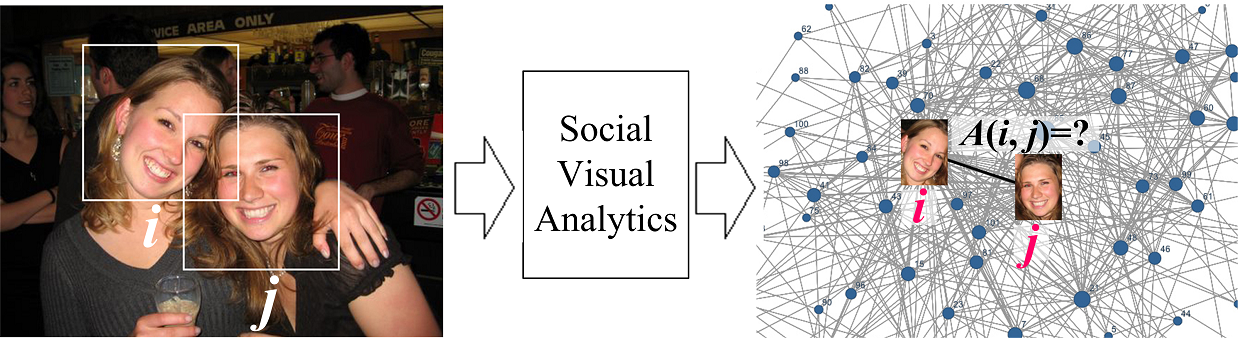
\includegraphics[width=\columnwidth]{intro}
\end{center}
\vspace{-0.25in} \caption{\captionsize 
(a-1) Original picture with detected faces; (a-2) relative positions of the detections; (a-3) Facial expressions; (a-4) Mutual Gazes; (a-5) Mutual poses; (a-6) scene recognition. (b-1) Independently recognizing the two faces: The right face is hard to distinguish between two possible people; (b-2) Recognizing faces using social relationship inferred from (a-1) through (a-6): The right face is now more likely to be associated with one person than the other. \label{fig:prob1}\afterfigspace}
\end{figure}

The example, as well as similar findings \cite{Gallagher,Wang2010,Murillo2012}, is inspiring, in that it convinces us that we have been equipped with sufficient computer vision capabilities for still images: These functionalities provide us a set of \emph{socially informative visual patterns}, and a smart selection and leveraging of them reveals new `words' that has never been seen by computer vision. High-level social contexts sensed from images through these socially informative visual patterns may conversely have immeasurable potentials in pushing traditionally hard problems forward, as has been argued and proved \cite{Stone2008,Stone2010}, for example in the task of face recognition from online imageries: Consider that in recognizing the two faces detected in Fig. \ref{fig:intro} (a-1) the right face is hard to distinguish between `Susan' and `Helen' (see (b-1)). However, the inferred `friends' relationship suggests that the individual should belong to the left person's list of friends (see (b-2)), which includes only `Helen' but not `Susan'.


\begin{figure}[t!]
\begin{center}
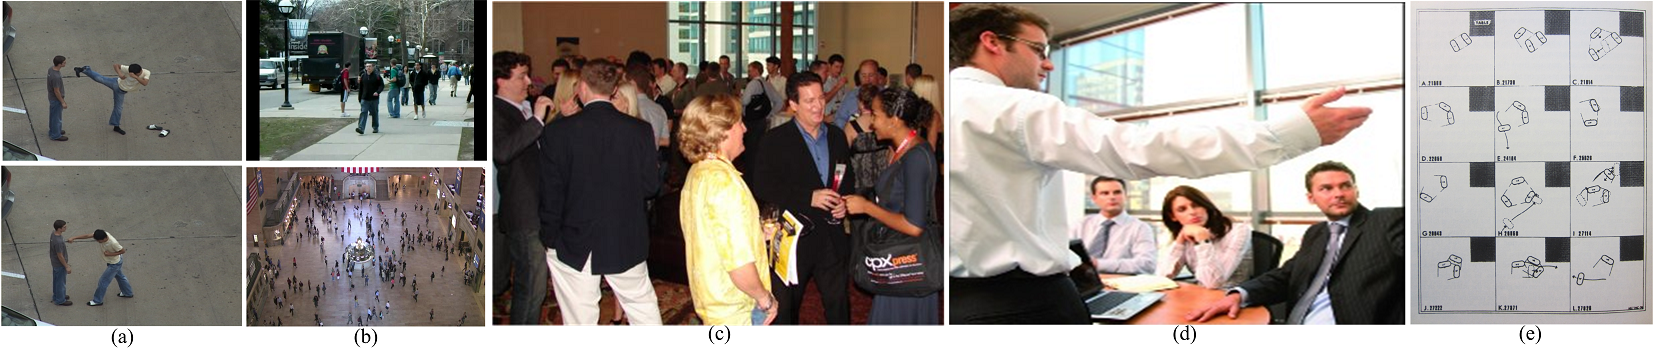
\includegraphics[width=\columnwidth]{socialbehavior}
\end{center}
\vspace{-0.25in} \caption{\captionsize 
(a): Socially non-informative co-occurrence of articulations\cite{UTdata}; (b): Socially non-informative collective crowd activities\cite{Choi:context,Choi:recogtrack}; (c): Socially informative salient interactions; (d) Socially informative salient group interactions in the nature; (e) Socially meaningful three-way activity categories defined as `f-formations' by sociology\cite{Kendon1990}.\label{fig:socialbehavior}\afterfigspace}
\end{figure}

Obviously, socially informative visual patterns not only exist in still images, but are also largely available from videos, where human behaviors are observed and recorded. While we may straightforwardly compute and represent the co-occurrences of multiple dynamic expressions, gazes, and poses, it however may not be necessarily true that these dynamic patterns are socially informative. To illustrate this, let us look at  a short video of co-occurrence of two-person actions, such as 'kick', 'punch', etc. (\cite{UTdata}, Fig. \ref{fig:socialbehavior}(a)),  where dynamics of the two people's poses and articulations can be extracted but they have limited extra implications beyond what we can tell from images. Similarly, the socially non-informative behavior patterns also include those group-wise or collective activities of a crowd, within which there are no explicit interactions, such as 'group-walking', 'queueing', etc. (\cite{Choi:context,Choi:recogtrack}, Fig. \ref{fig:socialbehavior}(b)).  Our common sense, on the one hand, implies that socially informative video patterns are more of gestural and conversational interactions, attention-response, as well as turn-taking meetings  (Fig \ref{fig:socialbehavior}(c)). On the other hand, sociology has provided well-defined socialization concepts, in terms of behavior categories, which has been proved in qualitative or quantitative sociological studies to be socially salient and meaningful, whose discovery however has not yet been automated by computer vision. Examples are in Fig. \ref{fig:socialbehavior} (e), which shows diagrams for such socially informative interaction categories, namely `f-formations', in three-way interactions that have been under the investigation of sociology.  


We seek to develop new approaches for detecting, localizing, and recognizing these socially informative visual patterns, i.e., interactions, from videos, in complementary to those companion efforts for still images. Through this effort, we foresee a richer set of heterogenous socially informative visual cues from videos in addition to those from images, so as to enable high-level reasoning as to be introduced in Section \ref{sec:vis2net}. We propose a paradigm as to be detailed in Section \ref{subsec:activity}, which is different from the existing work in three aspects. First, our approach is targeted to interactions that are defined and categories by dictionaries from sociology, but also generic to accommodate arbitrarily specified categories of interest and categories learned from data (Section \ref{sec:actlearn}), as well as interactions in social populations in the nature (Fig. \ref{fig:socialbehavior}(d)). Second, we builds upon realistic videos `in the wild', where the social interactions occur in unconstrained environment in the format of long-term surveillance videos of public areas, with irrelevant human beings co-existing with socially engaged actors as well as scene/background clutter. Our approach will be one that can effectively and efficiently localize and retrieve salient social interactions in space and time from these large volumes of cluttered image sequences. Third, realistic visual materials such as surveillance videos and web videos are frequently in low and varying frame-rate, in low resolution, blurry, as well as in adverse view-points. Our effort will be handling all these realistic conditions and providing robust and practical tools that process more than those simulated, high-quality, manually pre-processed data \cite{UTdata,Choi:context,Choi:recogtrack}.


%Second, we propose to predict activities under social contexts. In this case, social semantics assist in visual understanding in the way that they serve as contextual information for restricting the more possible categories of activities that may occur between a specific group of individuals. This effort is also complementary to the usage of social contexts for identifying the targets presented in the previous section. Consider a simple illustrative example in which we would like to label a conversational scene in a movie as either a `negotiation� or a 'debate'. It is possible, in this case, that by the analysis of facial expressions, gestures, and poses, we still have difficulty in distinguishing the two. However, by appropriate face recognition in association with other metadata of the movie, probably with the help of social contexts as introduced in the previous section, we may gain solid confidence regarding the social relationship between the speakers as either `cooperative' or 'adverse'. A cooperative relationship are more likely to imply a negotiating activity, and an adverse relationship implies otherwise. A mechanism, similar to and in companion to the CRF formulation but adapted to video analysis, will be particularly useful.


\subsubsection{Detection and recognition of interactions via matching}
\label{subsec:activity}

To detect a socially informative interaction and recognize its category, we propose an approach where the the interactions of interest are stored as exemplars in a gallery, each exemplar associated with a category label. As illustrated in Fig. \ref{fig:diagram_dataset}(a), our approach is based on matching. Given an exemplar video of a social interaction involving a small handful ($N$) of agents, we detect and localize instances of similar interactions within the long video of a larger gathering/clutter (i.e., $M\ge N$ people), and recognize their categories by matching the video against all the labeled exemplars and then extracting a category label or ranked list of labels from the resulting top-matches. We represent a social interaction as an ensemble of two types of time-varying descriptors: per-agent descriptors that encode the appearance and/or motion of each agent, and relative pairwise descriptors that encode the appearance and/or motion of each agent relative to another. Matching an exemplar interaction then amounts to searching through space and time for ensembles that are similar in some sense. This approach avoids generating explicit semantic descriptions of social interactions, and it is advantageous when one lacks the vocabulary to precisely describe a class of interactions, or when they cannot easily be broken down according to any pre-defined grammar.

\begin{figure}[t!]
\begin{center}
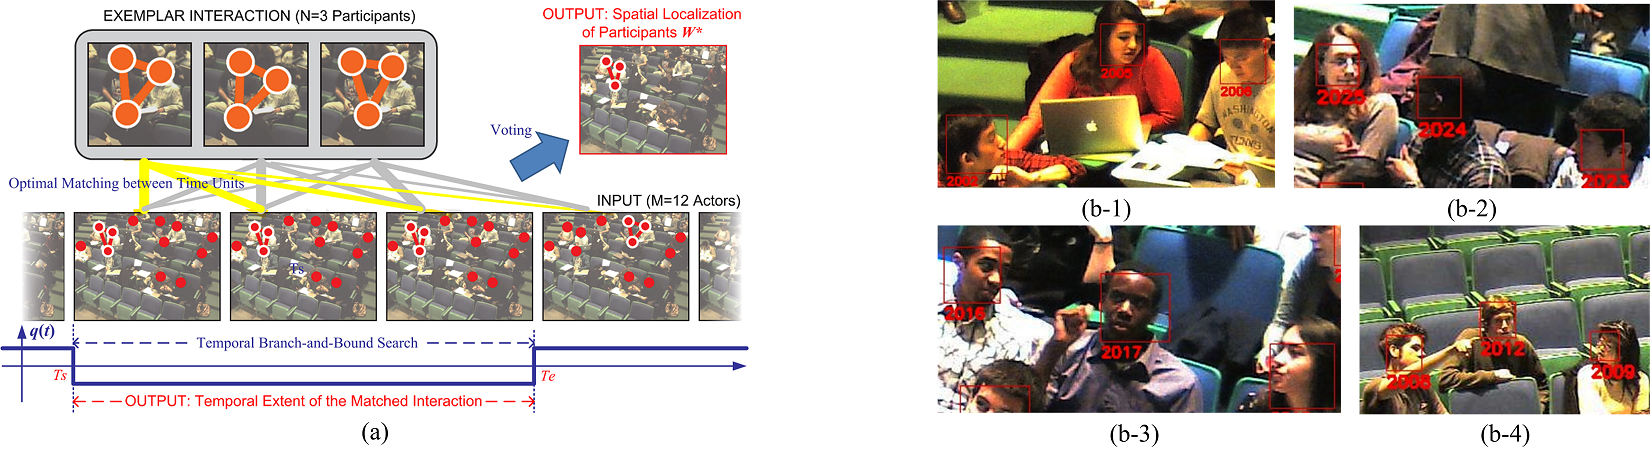
\includegraphics[width=\columnwidth]{diagram_dataset}
\end{center}
\vspace{-0.25in} \caption{\captionsize 
(a): The diagram illustration of the proposed approach for social interaction detection and recognition; (b-1)-(b-3): Examples of the three categories for two-person interactions; (c-1)-(c-4): Examples of the four categories for three-person interactions; (d) Example of the four-person interaction.\label{fig:diagram_dataset}\afterfigspace}
\end{figure}

More specifically, assume an input video consisting of $T$ frames. By applying domain-appropriate detection and tracking, assume we obtain $M$ space-time tracks of bounding boxes enclosing $M$ faces or bodies. The $M$ targets are to be compared with an interaction exemplar consisting of $S$ frames and $N$ targets that are correctly detected and tracked and all participating in an coherent interaction. Our representation for the input tracks therefore includes $M\times T$ $d_{I}$-dimensional descriptors $\{\mathbf{f}_{m,t}\}_{m=1,2,\cdots,M, t=1,2,\cdots,T}$, where $\mathbf{f}_{m,t}$ encodes the individual activity of the $m$th target at time $t$, and $M\times (M-1)\times T$ $d_{P}$-dimensional pairwise descriptors $\{\mathbf{g}_{m,m',t}\}_{m,m'=1,2,\cdots,M, m\neq m', t=1,2,\cdots,T}$, where $\mathbf{g}_{m,m',t}$ encodes dynamic visual properties of target $m$ exhibited relative to those of target $m'$ at time $t$. For each exemplar, we have two similar descriptor collections $\{\mathbf{f}^{D}_{n,s}\}_{n=1,2,\cdots,N, s=1, 2,\cdots, S}$ and $\{\mathbf{g}^{D}_{n,n',s}\}_{n,n'=1,2,\cdots,N, n\neq n', s=1, 2,\cdots, S}$. We denote the descriptor ensemble for the input at time $t$ to be $\mathcal{Q}_{t}\triangleq\{\mathbf{f}_{m,t},\mathbf{g}_{m,m',t}\}$, and that for the exemplar at time $s$ as $\mathcal{D}_{s}\triangleq\{\mathbf{f}^{D}_{n,s},\mathbf{g}^{D}_{n,n',s}\} $. The input is then represented as $\mathcal{Q}\triangleq\{\mathcal{Q}_{t}\}_{1\leq t\leq T}$ and the exemplar $\mathcal{D}\triangleq\{\mathcal{D}_{s}\}_{1\leq s\leq S}$.

Our tasks are 1) to identify from the $M$ targets in the input $N$ targets that demonstrate the most similar interactive pattern as the $N$ individuals in the exemplar, and 2) to temporally localize the extent of the interaction within the interval $[1, T]$. To formally describe task 1), consider the fact that if one of the $M$ targets is regarded as a participant in an interaction as exemplified by the exemplar $\mathcal{D}$, its behavior should properly match to the behavior of one of the $N$ individuals in the exemplar $\mathcal{D}$. Therefore, we use a $N\times M$ binary matrix $W=[w_{nm}]\in\{0,1\}^{N\times M}$ to formally represent the participant identification, where $w_{nm}=1$ means that the $n$th exemplar individual is matched to the $m$th input target and $w_{nm}=0$ means unmatched targets. For unambiguous matching, we expect each individual in the exemplar to find its unique partner target in the input. This implies that $\sum_{m}w_{nm}=1, \forall n$ and $\sum_{n}w_{nm}\leq 1, \forall m$, \textit{i.e.}, $W\mathbf{1}=\mathbf{1}$ and $\mathbf{1}^{T}W\leq\mathbf{1}^{T}$. Denote $\mathcal{W}\triangleq\{W\in\{0,1\}^{N\times M}| W\mathbf{1}=\mathbf{1}, \mathbf{1}^{T}W\leq\mathbf{1}^{T}\}$, and our former task is essentially to find $W^{*}\in\mathcal{W}$, which encodes the best matching between the input $\mathcal{Q}$ and the exemplar $\mathcal{D}$. To formally describe task 2) is straightforward: We simply look for the starting time $T_{s}$ and ending time $T_{e}$, $1\le T_{s}<T_{e}\le T$, such that the interactive pattern of input $\mathcal{Q}$ during $[T_{s}, T_{e}]$ demonstrates the best similarity with the exemplar $\mathcal{D}$.

Suppose that there are Mahalonobis-parameterized atomic distances $d_{I}(\mathbf{f}, \mathbf{f}')=(\mathbf{f}-\mathbf{f}')^{T}\Sigma_{I}(\mathbf{f}-\mathbf{f}')$ and $d_{P}(\mathbf{g}, \mathbf{g}')=(\mathbf{g}-\mathbf{g}')^{T}\Sigma_{P}(\mathbf{g}-\mathbf{g}')$ ($\Sigma_{I}\succeq 0$ and $\Sigma_{P}\succeq 0$ are positive semi-definite matrices) to compare descriptors, and accordingly define the `instantaneous' matching between input $\mathcal{Q}_t$ and exemplar $\mathcal{D}_s$ under matrix $W$ can be defined as 
\begin{equation}
\hat{D}(\mathcal{Q}_{t}, \mathcal{D}_{s}, W)=\sum_{nm}w_{nm}d_{I}(\mathbf{f}_{m,t}, \mathbf{f}^{D}_{n,s})+\!\!\!\!\!\!\sum_{nmn'm'}\!\!\!\!\!w_{nm}w_{n'm'}d_{P}(\mathbf{g}_{m,m',s}, \mathbf{g}^{D}_{n,n',t}).
\end{equation}
Consequently, the optimal instantaneous matching between input $\mathcal{Q}_t$ and exemplar $\mathcal{D}_s$ straightforwardly becomes $W^{t,s}\triangleq\arg\min_{W\in\mathcal{W}}\hat{D}(\mathcal{Q}_{t}, \mathcal{D}_{s}, W)$, and the ensemble distance between them becomes $D(\mathcal{Q}_{t}, \mathcal{D}_{s})\triangleq\min_{W\in\mathcal{W}}\hat{D}(\mathcal{Q}_{t}, \mathcal{D}_{s}, W)$. As a result, our approach, as illustrated in Fig. XXX, firstly evaluates all $T\times S$ ensemble distances $D(\mathcal{Q}_{t}, \mathcal{D}_{s})$ together with their 'instantaneous optimal matching' $W^{t,s}$ $\forall 1\le t\le T, 1\le s\le S$. This is followed by a Hough voting procedure to find the best matching $W^{*}$ from all instantaneous optimal matchings $\{W^{t,s}\}$. Finally, we construct from all ensemble distances $\{D(\mathcal{Q}_{t}, \mathcal{D}_{s})\}$a quality function $q(t)$, which achieves a negative value if and only if $t$ falls into the interval where the interaction of interest occurs, and therefore enable an efficient branch-and-bound search estimates the temporal extent $[T_{s}, T_{e}]$.  

\begin{figure}[t!]
\begin{center}
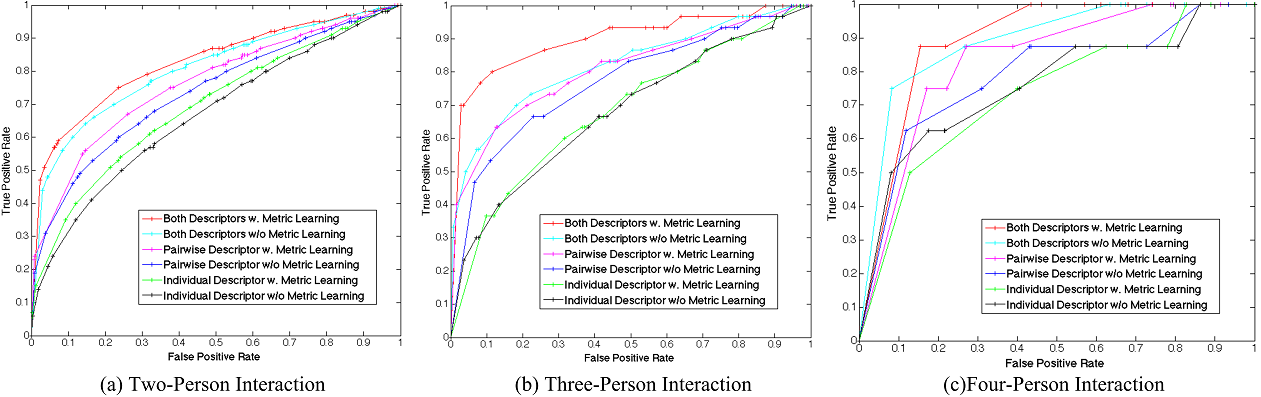
\includegraphics[width=\columnwidth]{ROC}
\end{center}
\vspace{-0.25in} \caption{\captionsize 
ROC curves for interaction detection using our proposed approach.\label{fig:dataset_compare}\afterfigspace}
\end{figure}

With the prototype system to be introduced in Section \ref{sec:sys}, we have successfully collected and processed a large-scale classroom behavior database consisting of 100 video clips in total. The classroom is ``interactive'' because at various times throughout the lecture students are invited to engage in ad-hoc group discussions about problems provided by the instructor. The scale of our database is orders of magnitude larger than state-of-the-art computer vision datasets (e.g. those used in \cite{UTdata,Choi:context,Choi:recogtrack}), in the number of individuals (10-50 students per camera), the number of cameras (6), and the amount of time (100 minutes per camera, per recording, equaling over 3,000 minutes in total). Through a combination of face detection and tracking, we obtained noisy tracks for all students in each monocular video, upon which we developed descriptive modules that directly extract descriptors for head pose (as individual per-agent descriptor) and body motion (as pairwise descriptor). We manually identified the participants and start/end times of all two-person, three-person, and four-person interactions, obtaining 254 two-person, 112 three-person, and 16 four-person interactions in total. In consultation with education experts we define interaction categories based on the geometric configurations of the participants: three categories for 2-person interactions (same row; different rows with left agent in front; different rows with right agent in front) and four categories for 3-person interactions. Example images for each category can be found in Fig. \ref{fig:diagram_dataset}(b)(c)(d). The annotated interactions range from a few seconds to tens of seconds in length. Since the raw videos arise from five different hour-long session, and we adopt a leave-one-session-out evaluation scheme in partitioning training/gallery samples (exemplars) from test samples (inputs). As our modules include both pose descriptors and relative motion descriptors, and our approach allows to learn optimal representations (in the form of metric learning (ML), see Section \ref{sec:actlearn}), To evaluate the effectiveness of all these functionalities, we turned off some of components as baselines and compared with the full module with all components on. Fig. \ref{dataset_compare} shows the ROC curves of the detection performance for the two-way, three-way, and four-way interactions. As expected we see that performance improves when more parts of the system turned on, which implies that our proposed approach has achieved promising technical quality.

In our following research, we aim to enrich the descriptions of the social behaviors in the current prototype system, explore more accurate and robust comparison and retrieval mechanisms, and in particular, design novel modules for integrating social contextual annotations to allow our framework to be fully `socially-aware'.


%%%%%%%%%%%%%%%%%%%%%%%%%%%%%%%%%%%%%%%%%%%%%%%%%%%%%%%%%%%%%%%%%%%%%%%%%%%%%%%%%%%%%%%%%%%%%%%%%%%%%%%%%

%\subsection{Joint Recognition of Multiple Targets with Social Contexts}
%\label{sec:recognition}
%
%The automatic recognition of targets in image and videos is an central task of computer vision. Recognition of objets is not only essential to any system that seeks to manage visual media based on content, but also necessary for automatically annotating images/videos (`auto-tagging') and indexing them. Recognition of faces is even integral to successfully interpreting images/videos of humans and consequently mining the social semantics in these imagery.
%
%Automatic recognition, since its initial stage until most recently, treats the targets as well as the outputted categories to be independent rom one to the other, which is essentially not the case. In order for automatic recognition to truly succeed, we must exploit the syntactic relationships between targets and between categories and use other contextual information. We in this section propose a scalable computational framework for socially-aware recognition systems that exploit contextual information from online social networks. These online communities provide two significant types of information which, to date, have only been scarcely exploited: 1) significant textual metadata, and 2) social network structure as context. The proposed activity seeks computational foundations for exploiting both.
%
%A typical example of socially-aware face recognition is as follows. A user uploads a small, hundred-image `album' (say)  and we seek to automatically recognize the identities of detected faces in the images. To achieve this goal, we represent the detected faces as nodes in a densely connected, undirected graph. With this representation, recognition consists of estimating a joint labeling of the nodes, which can be formulated as the optimization of an energy-based model. What is unique to our approach is that we seek energy models that combine image information (e.g., classifier output) with contextual information drawn from the user's online social network. Another example is scene recognition, where we seek to jointly label all images with their scene categories in several related online album containing thousands of scene images. Similar examples are more than the two mentioned examples.
%
%The description of an individual target is generally in multiple `views', where a view refers to a specific type of attribute that describes the target. A detected face, for example, can be described by skin color, texture, shape configurations of facial organs, etc.. The description of the contextual network relationship, meanwhile, is also in multiple views. The context between two faces(humans) in Facebook, for example, can be number of their shared friends, the number of their co-occurrence, and their relative poses in images, and so on. As we have mentioned, the social networks are usually partially observed, meaning that not all these views are `visible', and a practically useful recognition system must accommodate the un-observed views for the nodes or the links. Formally,  we can represent  the densely connected, undirected graph as $G$ describing the community of $K$ individuals, where $G\triangleq\{N^{(v_1)},A^{(v_2)},P^{(v_1)}, Q^{(v_2)}\}, v_1=1,2,\cdots,V_1,\hspace{5pt} v_2=1,2,\cdots,V_2$,  $N^{(v_1)}$ is a $K\times 1$ vector describing the individuals in the $v_1$th view, $P^{(v_1)}$ is a $K\times 1$ binary vector describing the visibility for that view, $A^{(v_2)}$ is the $K\times K$ affinity matrix describing the relational context for the $v_2$th view, and $Q^{(v_2)}$ is the $K\times K$ visibility matrix for that view. If $P^{(v_1)}(i)=1$, then $N^{(v_1)}(i)$ is the scalar description of the individual $i$ in the $v_1$th view; otherwise if $P^{(v_1)}(i)=0$ then $N^{(v_1)}(i)$ is a missing number indicating the lack of information of this node in this view. Similar notions apply for the matrices $A$ and $Q$.
%
%With this formulation, a natural computational framework for this socially-aware recognition is a conditional random field (CRF) model~\cite{lafferty2001crf, sutton2007icr, he2004mcr} with a node for each item of interest and an edge connecting many pairs of nodes. In this case, the goal is to infer a joint labeling $\vy=\{y_i\}$ of the relevant categories over all nodes $i$ in the graph. We use the notation $y_i\in{\cal L}=\{l_0\ldots l_M\}$ for the discrete label space of the nodes. (In general, these will vary from node to node, but we use a single set of labels here for notational convenience.) An optimal joint labeling is found by maximizing the conditional density
%\begin{equation} \label{eq:crf}
%{\rm Pr}(\vy|G) = \frac{1}{Z(G)}e^{-E(\vy|G)}
%\end{equation}
%where the partition function $Z(G)$ is a data-dependent normalizing constant and the energy $E(\vy|G)$ consists of sums of unary and pairwise potential functions at the nodes and edges:
%\begin{equation}\label{eq:energy}
%E(\vy|G) =  \sum_{i}  \phi_i (y_i|G) + \sum_{(i,j)} \phi_{ij}(y_i, y_j|G).
%\end{equation}
%
%In the CRF framework, the unary potential functions $\phi_i(y_i|G)$ capture information that is local to each node, and the pairwise potentials $\phi_{ij}(y_i, y_j|G)$ represent the compatibilities of possible label pairs across an edge. Therefore, assuming that the unary potentials depend on individual descriptions and pairwise potentials depend on contextual descriptions, (\ref{eq:energy}) can be decomposed as
%\begin{equation}\label{eq:energy_simple}
%E(\vy|G) =  \sum_{i}  \phi_i (y_i|N,P) + \sum_{(i,j)} \phi_{ij}(y_i, y_j|A,Q).
%\end{equation}
%As part of the proposed activity, we will study the application of this model to practical recognition tasks. Our goal is to answer the following three questions: 1) what types of social network context information improve recognition and by how much?; 2) how should multiple-view of information be weighted and how should missing observation be accounted for?; and 3) how can we apply this model at a practical scale? 
%
%\begin{figure}[t!]
%\begin{center}
%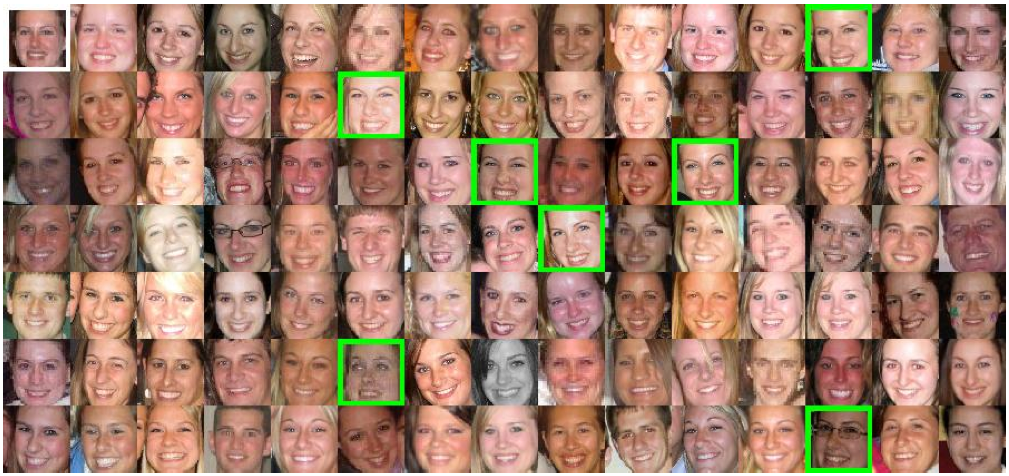
\includegraphics[width=3.5in]{ivw_facescores}
%\end{center}
%\vspace{-0.25in} \caption{\captionsize 
%The performance of a commercial face recognition system on tagged faces harvested from Facebook~\cite{Stone2008}. Given the query face in the upper left, the system has returned the remaining faces as being most similar. Similarity to the query decreases from left to right and from top to bottom, and the ground-truth matches are highlighted with green squares. Due to the variability of this `real-world' dataset, the correct matches are not highly ranked.\label{fig:face-results}\afterfigspace}
%\end{figure}
%
%
%
%\SubSubSection{Preliminary Study}\label{sec:prelim-face-results}
%Evidence for the utility of social network context is provided under simplified assumptions by the work of PI Zickler~\cite{Stone2008,Stone2010}, the former of which received the Best Paper Award at the First IEEE Workshop on Internet Vision. This work reported the results of a preliminary study on the ability of social network context to improve face-based identity recognition using a subset of 2641 labeled faces from Facebook. In this study, we restricted our attention to images with two faces (two-node graphs) so that CRF training and inference could be achieved without approximation. The label space ${\cal L}=\{l_0,\ldots,l_M\}$  consists of a set of possible identities, and we considered a simple set of individual node descriptions and contextual relationship descriptions. Specifically, we assumed that all descriptions in all views are observed and error-free, in which case the potentials in (\ref{eq:energy_simple}) are further expanded as a linear combination of view-specific univariate and bivariate \emph{feature functions} independent of observability variables $P,Q$:
%\begin{eqnarray}
%\phi_i(y_i|N,P) &=& \sum_{v_1} \alpha_{v_1}(N^{(v_1)}) f_{v_1}(y_i, N^{(v_1)})\\
%\phi_{ij}(y_i, y_j|A,Q) &=& \sum_{v_2} \beta_{v_2}(A^{(v_2)}) g_{v_2}(y_i, y_j, A^{(v_2)}).
%\end{eqnarray}
%
%
%\begin{figure}[t!]
%\begin{center}
%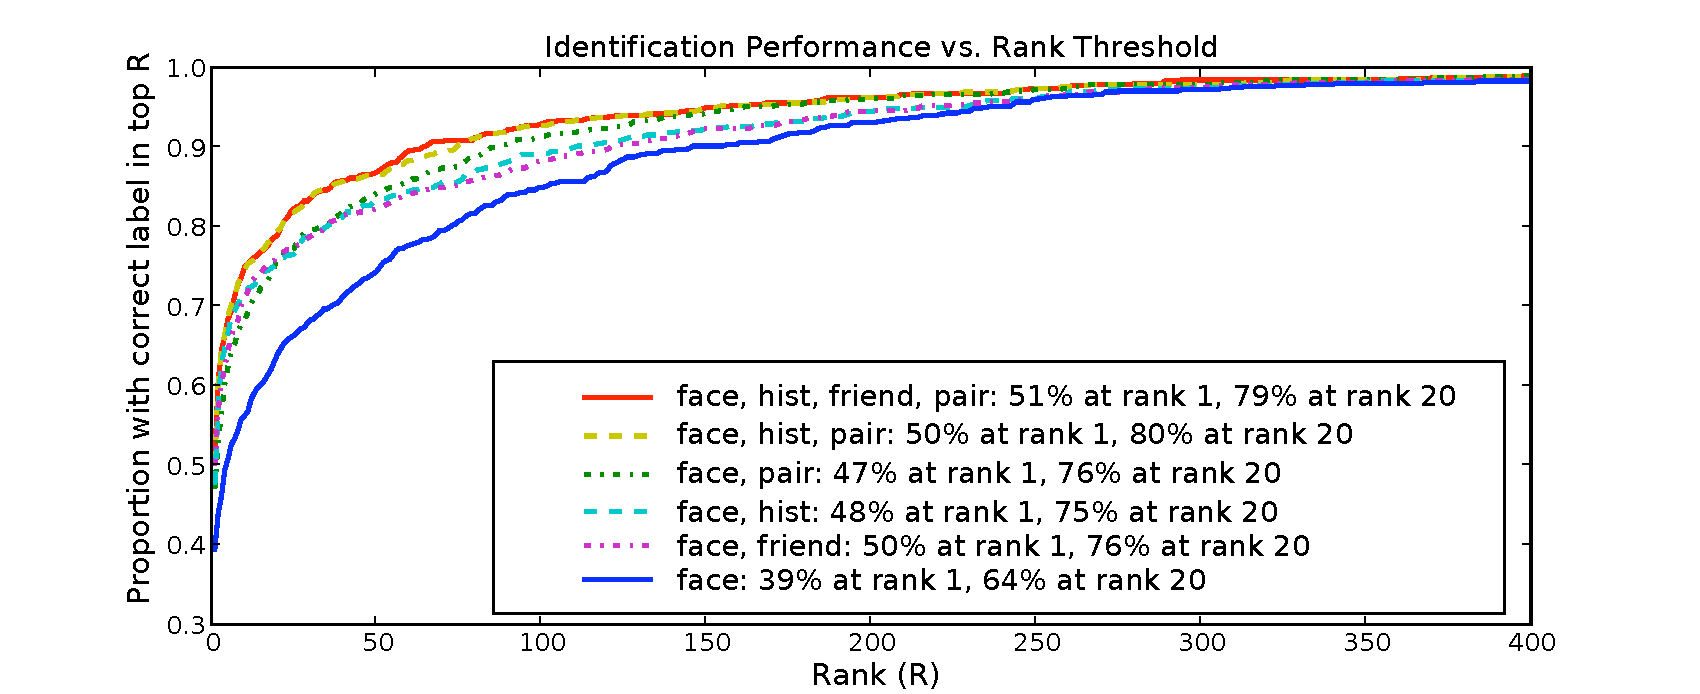
\includegraphics[width=5in]{rank_graph_small}\\
%{\footnotesize
%\begin{tabular}{ll}
%\hline\hline\multicolumn{2}{l}{\raisebox{-0.1in}{Univariate Functions $f_{v_1}(y_i, N^{(v_1)})$}} \\
%\hline
%\parbox[t]{1.8in}{\raggedright Face score (\textsf{face})} & \parbox[t]{3.5in}{A distribution of likelihoods over ${\cal L}$ returned by a commercial face recognition system (see Fig.~\ref{fig:face-results})} \vspace{0.03in}\\
%\parbox[t]{1.8in}{\raggedright Photo history (\textsf{hist})} & \parbox[t]{3.5in}{Number of times each individual $l_m$ has been tagged in previous photos posted by the photographer} \vspace{0.07in}\\
%\multicolumn{2}{l}{Bivariate Functions $ g_{v_2}(y_i, y_j, A^{(v_2)})$} \\
%\hline
%\parbox[t]{1.8in}{\raggedright Friendship (\textsf{friend})}& \parbox[t]{3.5in}{Binary indicator that is one iff individuals $l_m$ and $l_n$ are `Facebook friends' } \vspace{0.04in}\\
%\parbox[t]{1.8in}{\raggedright Pairwise co-occurrence (\textsf{pair})}& \parbox[t]{3.5in}{Number of times each pair of individuals $(l_m,l_n)$ has been jointly tagged in previous photos posted by the photographer}\\
%\end{tabular}}
%\end{center}
%\captionspace \caption{\captionsize 
%Face recognition performance as a function of rank threshold for a variety of combinations of feature functions (described bottom). At each rank value $R$, the graph displays the proportion of all test samples for which the correct ground-truth identity label appeared in the top $R$ predictions. Social network context improves recognition, and different sources of context information are complimentary\cite{Stone2008}.\label{fig:ivw-curves}\afterfigspace}
%\end{figure}
%
%
%The results are summarized in Figs.~\ref{fig:face-results} and \ref{fig:ivw-curves}. For each combination of feature functions, we determined model parameters ($\alpha$ and $\beta$) by maximizing the conditional log-likelihood of a training set by gradient ascent. Then, for each left-out test photo, exact marginal probabilities were computed for the test photo's face-nodes, and  the outputs were compared against ground truth. Specifically, the marginal probabilities were used to compute a ranked list at each node, and we measured how often the correct identity label appeared in the top $R$ ranks for a sliding value of $R$ (c.f.~\cite{frvt06}).
%
%A number of observations can be drawn from these results. First, even when using the face score (\textsf{face}) alone (see Fig.~\ref{fig:face-results}) social network context plays a vital role. In our data, over 99\% of tagged faces correspond to `friends' of the photographer, and since the identity of the photographer is known (it is included in the input $N$), we can safely reduce the label space ${\cal L}$ from the 15,752 individuals in the global gallery to the hundreds of friends of the input photographer. Without this restriction, the results in Fig.~\ref{fig:face-results} would degrade remarkably. The results in Fig.~\ref{fig:ivw-curves} also demonstrate that social network context substantially improves baseline face recognition, and that different sources of context information are complementary.
%
%
%These preliminary results are encouraging, especially since the network context information that was employed barely scratches the surface of possibilities. Existing work shows that clothing can provide useful information within an album~\cite{anguelov2007cir, zhang2003aah,  song2006cah, sivic2006fpr}, and it is possible that clothing could be used more globally as well, since the long-term clothing trends of certain individuals may be distinguishable from those of others. Recognition of facial attributes~\cite{LNCS53050340}, such as glasses or facial hair, can be used in conjunction with identity scores to improve recognition, and the same is true for gender recognition, which in many online communities is a knowable piece of information. In addition, people associate with each other in homes, schools, outdoors, workplaces, clubs, and so on, and a more explicit representation of these would be beneficial. Certain individuals will appear more often in certain types of scenes, and these `likely' scene types will change depending on who they are with. Temporal and geographic information, when available, may be further predictive of which individual is likely to occur and with whom. 
%
%
%
%In our proposed research, we aim to both qualitatively and quantitatively analyze large collections of images and their embedding network to discover the utility of these multi-view context information, and in particular, explore effective approaches to account for incompletely observed graph, which is the crucial to allow our framework to succeed in realistic network conditions.
\subsubsection{Learning social interaction detectors and categories}
\label{sec:actlearn}


Given a set of defined interaction categories, we can detect instances of these categories (and then extract useful information about the social network) using the methods of the previous section. But how do we learn the categories in the first place? How can we make use of labeled samples of interactions? What if no labeled samples are present? In this subsection, we show an initial attempt to use the proposed social interaction representation to maximize the performance of the social interaction detection and recognition method presented in Section \ref{subsec:activity}, and introduce our planned efforts on learning the social interaction categories in a semi-supervised as well as unsupervised manner before we can learn better detectors.


When supervision is available for the data used in Section \ref{subsec:activity}, we learn optimal interaction matching parameters, that is, symmetric semi-positive definite matrices $\Sigma_{I}$, $\Sigma_{P}$ for the atomic distances $d_I(\mathbf{f},\mathbf{f}')$ and $d_P(\mathbf{g},\mathbf{g}')$, so that the learned metrics can: 1) enhance discrimination between exemplar categories by ensuring that distances are smaller when descriptors are drawn from roughly the same temporal location within a labeled exemplar of the same category, and larger otherwise; and 2) enhance the accuracy of temporal localization by ensuring that distances between labeled ensembles and unlabeled ``background'' ensembles are large. The combination of 1) and 2) leads to more accurate spatial localizations of participants (\emph{i.e.}, better matching matrix $W^{*}$), and induces the ``quality function'' for efficient temporal localization. To do so, we may construct two collections from our database exemplars. The collection $\mathcal{P}$ contains all pairs of instantaneous interaction ensembles that are of the same category and occur roughly in the same temporal location within the interaction instances, together with their ``ground-truth" matchings. The collection $\mathcal{M}$, on the other hand, is comprised of ordered triples $(h,k,l)$ in which ensemble $h$ is the same category as ensemble $k$ and ensemble $l$ is either of a different category or background. Having defined these two collections, the Mahalanobis parameters are found by solving
\begin{equation}
\label{classify}
\begin{split}
&\min_{\Sigma_{I}, \Sigma_{P}} \sum_{(u,v)\in\mathcal{P}}\hat{D}(\mathcal{D}_{u}, \mathcal{D}_{v}, W_{u,v})+\gamma\sum_{(h,k,l)\in\mathcal{M}}\xi_{h,k,l},\\
&\textup{s.t.}  \hat{D}(\mathcal{D}_{h}, \mathcal{D}_{l}, W)-\hat{D}(\mathcal{D}_{h}, \mathcal{D}_{k}, W_{h,k})\ge 2-\xi_{h,k,l}, \Sigma_{I}\succeq 0, \Sigma_{P}\succeq 0, \xi_{h,k,l}\ge0,
\end{split}
\end{equation}
where $W_{u,v}$ is the ``ground-truth" matching for pair $(u,v)$ and $W$ is an arbitrary matching. The minimization over either $\Sigma_{I}$ or $\Sigma_{P}$ is exactly a Large Margin Nearest Neighbor (LMNN) problem \cite{Weinberger:ML}, and we apply LMNN multiple times to separately learn one distinct pair of ($\Sigma_{I}, \Sigma_{P}$) for each value of the number of interaction participants. 



The task of unsupervised or semi-supervised learning of new categories has a major challenge and a major advantage. Technically, social interactions involve multiple agents and are mostly represented as descriptor ensembles,   and correspondences between an agent in one ensemble and another agent in the other ensemble are crucial in accurately characterizing the similarity or distance between two ensembles. Therefore, the semi-supervised or unsupervised discovery will operate on ensembles of vectors with (structural) correspondence effects taken into account. The clustering of ensembles (sets) with ensemble distance involving structural correspondence has only received scarce, if not no, treatment from either computer vision or machine learning. On the other hand, in many situations the visual information is accompanied by other textual metadata where the social semantics are implicitly embedded: Contemporary online photo albums are largely tagged, and our interactive classroom is also equipped with a teaching-learning database where the students' social connections can be derived or inferred (see Section \ref{sec:sys}). These contextual information will be particularly useful, in providing side-supervisions to the raw visual materials. These implicit supervision can be regarded, for example, as the same network exhibited in another `domain' than the `visual domain', and consequently can be exploited in a similar manner as our recent contribution on domain adaptation \cite{LiZickler2012,Li2011}. In our proposed effort for semi-supervised and unsupervised learning of interaction representations, the challenge and the advantage will both be situated in central position. 



%%%%%%%%%%%%%%%%%%%%%%%%%%%%%%%%%%%%%%%%%%%%%%%%%%%%%%%%%%%%%%%%%%%%%%%%%%%%%%%%%%%%%%%%%%%%%%%


%\subsection{Salient Social Activities Discovery and Prediction}
%\label{sec:activity}
%
%The joint target recognition problem described in the previous section represent one scenario where social contexts significantly assist and improve a traditional computer vision task. In this section, we propose a \emph{new} computer vision task motivated and enabled by socialized metadata. This new task introduces new `words' that a picture or a video may convey, and the output conversely produces new clues for social sensing in related disciplines. 
%
%As the second major problem regarding socially-aware visual understanding, we propose to discover and predict salient social activities from videos, as well as still images if possible. The proposed task is novel from existing activity analysis and recognition work in three aspects: It seeks to discover salient social behaviors,  it  aims to predict activities using social contexts, and it directly builds upon realistic visual materials `in the wild'.
%
%\begin{figure}[t!]
%\begin{center}
%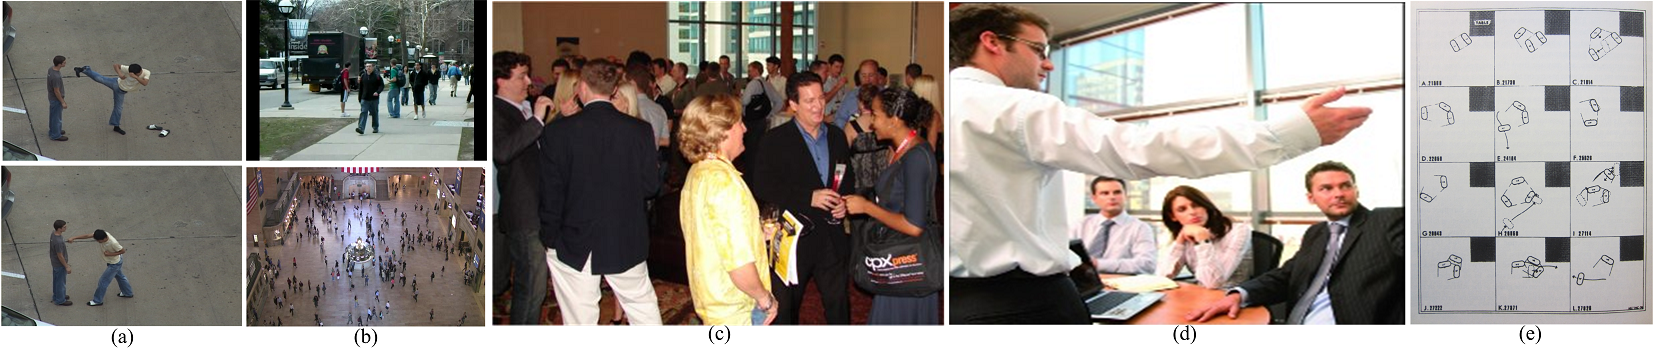
\includegraphics[width=\columnwidth]{socialbehavior}
%\end{center}
%\vspace{-0.25in} \caption{\captionsize 
%(a): Socially non-informative co-occurrence of articulations\cite{UTdata}; (b): Socially non-informative collective crowd activities\cite{Choi:context,Choi:recogtrack}; (c): Socially informative salient interactions; (d) Socially informative salient group interactions in the nature; (e) Socially meaningful three-way activity categories defined as `f-formations' by sociology\cite{Kendon1990}.\label{fig:socialbehavior}\afterfigspace}
%\end{figure}
%
%
%First, we propose to discover salient social activities. Specifically, social semantics assist in visual understanding in the way that they provide new social behavior categories for us to distill from images and videos, and these new social categories are informed by qualitative and quantitative sociology, which has been studying these behavior modes but never be automated by computer vision. As these new concepts are socially meaningful, they provide more expressive evidence about the social relationships among the individuals involved in the activities. We refer to these new social semantics as salient. In contrast to existing vision research, salient social activities are distinctive because they do not focus on non-informative interactions or group-wise behaviors. The non-informative interactions, for example, refer to the co-occurrences of two individual body articulations with limited clue about how the two individuals are related or exchange opinions, such as 'kick', 'punch', etc. (\cite{UTdata}, Fig. \ref{fig:socialbehavior}(a)). The non-informative group-wise behaviors, on the other hand, include collective activities of a crowd, within which there are no explicit interactions, such as 'group-walking', 'queueing', etc. (\cite{Choi:context,Choi:recogtrack}, \ref{fig:socialbehavior}(b)). Instead, the salient social activities are more  of gestural and conversational interactions, attention-response, as well as turn-taking meetings  (Fig \ref{fig:socialbehavior}(c)) where sociological semantics, as is interesting and important to the sociology research, can be derived. Fig. \ref{fig:socialbehavior} (e) shows diagrams for such socially meaningful activities categories, namely `f-formations', in three-way interactions that have been under the investigation of sociology. Moreover, we will develop generic salient socialized discovering models and approaches, so that they accommodate activities of social populations of animals and insects (Fig. \ref{fig:socialbehavior}(d)).
%
%Second, we propose to predict activities under social contexts. In this case, social semantics assist in visual understanding in the way that they serve as contextual information for restricting the more possible categories of activities that may occur between a specific group of individuals. This effort is also complementary to the usage of social contexts for identifying the targets presented in the previous section. Consider a simple illustrative example in which we would like to label a conversational scene in a movie as either a `negotiation� or a 'debate'. It is possible, in this case, that by the analysis of facial expressions, gestures, and poses, we still have difficulty in distinguishing the two. However, by appropriate face recognition in association with other metadata of the movie, probably with the help of social contexts as introduced in the previous section, we may gain solid confidence regarding the social relationship between the speakers as either `cooperative' or 'adverse'. A cooperative relationship are more likely to imply a negotiating activity, and an adverse relationship implies otherwise. A mechanism, similar to and in companion to the CRF formulation but adapted to video analysis, will be particularly useful.
%
%Third, we expect to develop approaches that directly take in realistic visual materials recording social activities of interest. On the one hand, realistic visual materials capture the social activities in unconstrained environment in the format of long-term surveillance videos of public areas with irrelevant human beings co-existing with socially engaged actors as well as scene/background clutter. Our approach will be one that can effectively and efficiently localize and retrieve salient social activities in space and time from these large volumes of cluttered image sequences. On the other hand, realistic visual materials such as surveillance videos and web videos are frequently in low and varying frame-rate, in low resolution, blurry, as well as in adverse view-points. Our effort will be handling all these realistic conditions and providing robust and practical tools that process more than those simulated, high-quality, manually pre-processed data \cite{UTdata,Choi:context,Choi:recogtrack}.
%
%\subsubsection{A prototype system and preliminary results}
%
%\begin{figure}[t!]
%\begin{center}
%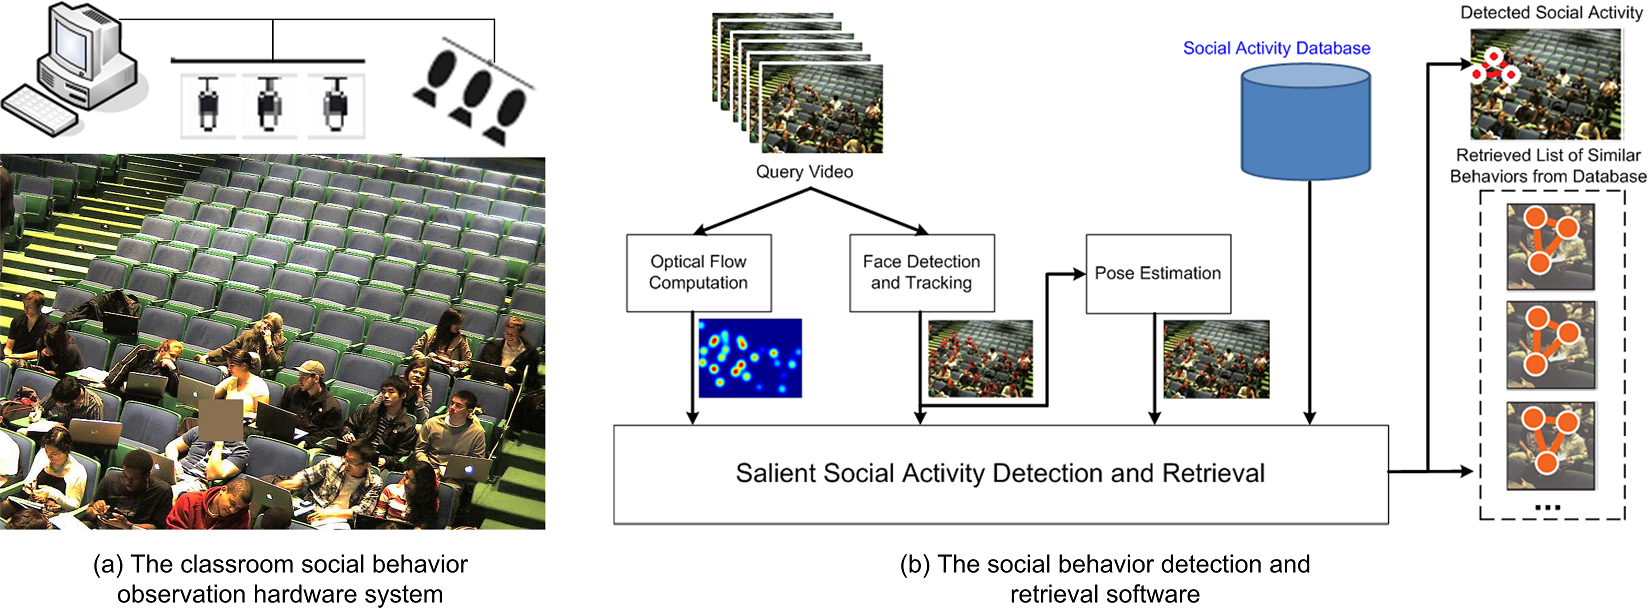
\includegraphics[width=\columnwidth]{prototype}
%\end{center}
%\vspace{-0.25in} \caption{\captionsize 
%The prototype hardware and software infrastructure for analyzing socialized human behaviors in an indoor environment at Harvard University.\label{fig:prototype}\afterfigspace}
%\end{figure}
%
%As an initial attempt to analyze socialized human behaviors in an indoor environment, we have built up a prototype hardware and software infrastructure at Harvard University. As shown in Fig. \ref{fig:prototype}(a), the hardware part of the prototype system mainly consists of a networked audio-visual recording system for large-scale recording of student interactions in a Harvard College lecture hall. The system records audio and video from approximately one hundred students during each lecture in conjunction with the audience responses through an online teaching-learning application. The video system uses six IP cameras that together provide resolution that is high enough to achieve face-based identity recognition of each student in the audience. The audio system is an innovative design consisting 48 omnidirectional boundary microphones mounted inconspicuously among the seats, and outputting sound from each microphone recording to a single user-friendly mp3 audio file.To automatically analyze the videos, we have developed a robust computational suite of computer vision tools. This software consists of several fundamental modules that directly distill behavioral descriptions from raw videos, as well as a high-level module that detects salient social activities of interest from a new video and retrieves similar social activities. 
%
%
%With this established classroom observation system and these fundamental modules, we have successfully collected and processed a large-scale classroom behavior database consisting of 100 video clips in total. The students are seated in a regular lecture hall and are observed by a camera array with non-overlapping fields of view. The classroom is ``interactive'' because at various times throughout the lecture students are invited to engage in ad-hoc group discussions about problems provided by the instructor. The scale of our database is orders of magnitude larger than state-of-the-art computer vision datasets (e.g. those used in \cite{UTdata,Choi:context,Choi:recogtrack}), in the number of individuals (10-50 students per camera), the number of cameras (6), and the amount of time (100 minutes per camera, per recording, equaling over 3,000 minutes in total). Through a combination of face detection and tracking, we obtained noisy tracks for all students in each monocular video, upon which we developed descriptive modules that directly extract descriptiors such as head pose and body motion, we have also implemented a high-level module for behavior analysis based on similarity between two social groups, as depicted in Fig. \ref{fig:prototype}(b). In this module, the behavior of each individual is represented by a combination of the head pose and the motion of torso and arms (using the method of histogram of optical flows). The social behavior of a group is then represented by the configuration in space and time of the behaviors of its participants. With this social activity representation, the module detects a salient social activity from a new video and retrieves similar social activities from our established database. This functionality is illustrated in Fig. \ref{fig:prototype}(b), where our system has discovered a three-way conversation by identifying the participants of this conversation and the time span (several to tens of seconds) of this event. Based on the behavior representation for this space-time social interaction, the system searches the remainder of the database and retrieves a list of exemplars containing similar social behavior, ranked in the descending order of the similarities with the query. In this way, any manual annotations associated with the query video can be propagated to the top-ranking exemplars, and we are now taking this approach to propagate our manual annotations across the whole database. 
%
%
%\begin{figure}[t!]
%\begin{center}
%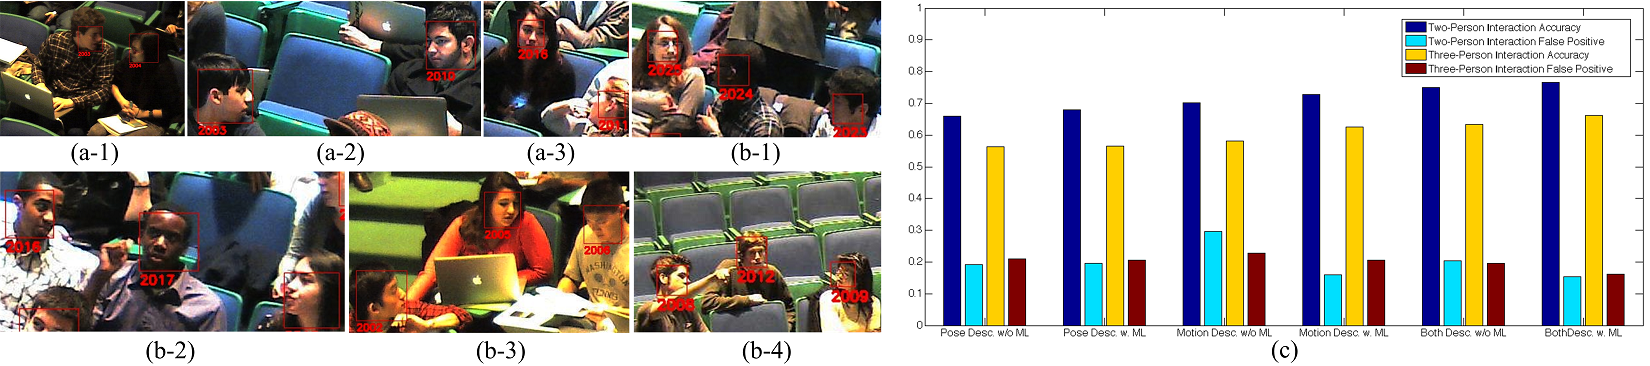
\includegraphics[width=\columnwidth]{dataset_compare}
%\end{center}
%\vspace{-0.25in} \caption{\captionsize 
%(a-1)-(a-3): Examples of the three categories for two-person interactions; (b-1)-(b-4): Examples of the four categories for three-person interactions; (c) Preliminary performance comparisons of our social activity retrieval software.\label{fig:dataset_compare}\afterfigspace}
%\end{figure}
%
%
%To evaluate the effectiveness of the social behavior retrieval module, we manually identified the participants and start/end times of all two-person, three-person, and four-person interactions, obtaining 254 two-person and 112 three-person interactions in total to constitute the entire database. In consultation with education experts we define interaction categories based on the geometric configurations of the participants: three categories for 2-person interactions (same row; different rows with left agent in front; different rows with right agent in front) and four categories for 3-person interactions. Example images for each category can be found in Fig. \ref{fig:dataset_compare}(a)(b). The annotated interactions range from a few seconds to tens of seconds in length. Since the raw videos arise from five different hour-long session, and we adopt a leave-one-session-out evaluation scheme in partitioning training samples (exemplars) from test samples (inputs). We study classification performance for 2-person and 3-person interactions, where we measure the accuracy of inferred interaction categories. Our low-level modules include both pose descriptors and relative motion descriptors, and our high-level module employs Metric Learning (ML). To evaluate the effectiveness of all these functionalities, we turned off some of components as baselines and compared with the full module with all components on. Fig. \ref{fig:dataset_compare}(c) shows the average true positive rates vs. false positives when classifying detected interactions into the three or four categories. As expected we see that performance improves when more parts of the system turned on, which implies that our prototype infrastructure has achieved reasonable technical quality.
%
%In our proposed research, we aim to enrich the descriptions of the social behaviors in the current prototype system, explore more accurate and robust comparison and retrieval mechanisms, and in particular, design novel modules for integrating social contextual annotations to allow our framework to be fully `socially-aware'.
% !TEX root = SocialVision2012.tex

\subsection{Multi-source multi-view network estimation}
\label{sec:vis2net}

In addition to analyzing social interactions in videos, we will investigate tools for analyzing social \emph{relationships}, in terms of the social network that embeds the people observed in an image and video collection. As is customary, we consider the social network of $K$ individuals to be an undirected weighted graph $G$, with $K$ nodes and a non-negative weight ($\in [0,1]$) on the edge between each node-pair. Each  weight represents the social proximity, or strength of tie, between two people, and the weights are collected in a positive symmetric affinity matrix $A$ of size $K\times K$. As described in Sections~\ref{sec:intro} \& \ref{sec:background}, our goal is to develop network reconstruction methods that are well-suited for vision by simultaneously: 1) modeling the multiple-community structure of social networks; 2) incorporating a variety of noisy sources (i.e., social cues automatically extracted from images and videos of varying quality); and 3) tolerating identity errors and high levels of missing data.

It has commonly been observed that social networks include multiple overlapping communities (e.g.,~\cite{AiroldiBFX08,Kim12}). Computationally, this means that the social proximity between nodes is not scalar-valued but depends on the type of roles or memberships (e.g., friends vs. workmates vs. family) by which it is being considered. We refer to these communities as different \emph{views} in the network and we represent them by defining $G\triangleq\{A^{(v)}\}_{v=1}^{V}$, where $A^{(v)}$ is the affinity matrix summarizing the ties between every pair of nodes as measured in the $v$th view. For example, if $v\in\{1,2,3\}$ corresponds to friends, family, and workmates,  $A^{(1)}(i,j)=1$, $A^{(2)}(i,j)=0$, and $A^{(3)}(i,j)=1$ indicates that Alice ($i$) and Bob ($j$) are unrelated but are simultaneously close friends and workmates. 
%The multiple views overlap in general, and the effective tie between each node pair depends on which view is be used to assess their relationship.

In addition to considering multiple views, we will also account for social information coming from multiple distinct cues extracted from visual data, without these cues being associated with peoples' identities with complete certainty. To do this, we consider $S$ \emph{sources} producing socially-informative cues $\vy^s, s=1,2,\cdots,S$, with each $\vy^s(i,j)$ being a multi-dimensional descriptor computed from a distinct socially-informative visual cue related to person $i$ and person $j$. As an example, for a detected, tracked and correctly-identified pair of individuals Alice $(i)$ and Bob $(j)$, a set of sources could include (time-varying in videos): relative positions of the two detections $\vy^1(i,j)$ (or $\vy^1$ for short);  relative head poses $\vy^2$; relative body poses $\vy^3$; distribution over interaction categories $\vy^4$ recovered as in Section~\ref{sec:activity}; and scene category $\vy^5$. These cues will not generally be associated uniquely with one pair of individuals because of uncertainties inherent to face recognition and other forms of identity recognition, and this means that
each source will generally produce from the same image or video sequence multiple differently-weighted outputs. For example, if we cannot visually distinguish Bob ($j$) from Charlie ($k$) then each source will produce from one video sequence two outputs that satisfy $\vy^s(i,j)=\vy^s(i,k)$. 

\boldstart{Restricted regression}. \todd{I just made up this name. Can you think of a better one?} One of our project goals is to establish a unified, data-driven framework for reconstructing multi-view network representations (affinity matrices $A^{(v)}$) from multiple noisy, heterogeneous visual sources. We refer to this problem as multi-source multi-view network estimation, and we will address it using an architecture  comprised of $V$ trained \emph{oracles} $\Psi_{v}$ that each provide an estimate of one view $\hat{A}^{(v)}$ from all available vision-based descriptors $\bar{\vy}=[\vy^1,\vy^2, \cdots,\vy^S]$. That is, $\hat{A}^{(v)}=\Psi_{v}(\bar{\vy})$, with $\Psi_{v}$ learned from data according to the following general approach. Given collections of vision-based social cues $\{\bar{\vy}_{n}\}_{n=1}^{N}$ attributed to $N$ different unknown social network graphs, optionally supplemented by additional collections $\{\bar{\vy}_{n}\}_{n=1}^{M}$ attributed to $M$ graphs that are known (i.e., known 
affinity matrices $\{\bar{A}^{(v)}_{m}\}_{m=1}^{M}$, perhaps through non-visual metadata like that described in Section \ref{sec:sys}), we will investigate a family of objectives of the form
\begin{equation}\label{eq:sensing}
\{\Psi^{*}_{v}\}=\arg\!\!\!\!\!\!\!\!\min_{\{\Psi_{v}\},\{\hat{A}^{(v)}_l\}_{l=1}^{N+M}}\sum_{m=1}^{M}\mathcal{J}\left(\{\Psi_{v}\}, \{\bar{\vy}_m\}, \{\bar{A}^{(v)}_m\}\right)+\tau\left(\{\hat{A}^{(v)}_m\},\{\hat{A}^{(v)}_n\}\right)+\gamma\left(\{\Psi_{v}\}\right).
 \end{equation}
The first term $\mathcal{J}$ in this expression is a loss term that gives preference to oracles that agree with the $M$ known graphs. For example,  $\mathcal{J}(\{\Psi_{v}\}, \{\bar{\vy}_m\}, \{\bar{A}^{(v)}_m\})=\sum_{v=1}^{V}\|\Psi_{v}(\vy_m)-A^{(v)}_m\|^{2}$ would measure discrepancy from the known graphs in a least-squares sense. To prevent over-fitting, the complexity of the oracles is restricted by a regularization term $\gamma()$, whose form depends on the choice of regression machine, such as Gaussian process regression \cite{GPbook} or deep learning \cite{DLbook}. We will also explore modifying this regularization term to enforce compatibility between the oracles of different views. Two oracles predicting friendship and adversarialism for the same pair of nodes, for example, should be deemed incompatible. Finally, we include a third term $\tau()$ that regularizes the estimated affinity matrices according to some generic or environment-specific prior knowledge. For these, we will draw inspiration from the many existing statistical graph models~\cite{Goldenberg}.

In this thread of our research,  cross-view compatibility and within-view clustering are expected to play essential roles in the multi-view architecture. This distinguishes the proposed work from conventional regression machines, where outputs are mutually independent.

%\begin{figure}[t!]
%\begin{center}
%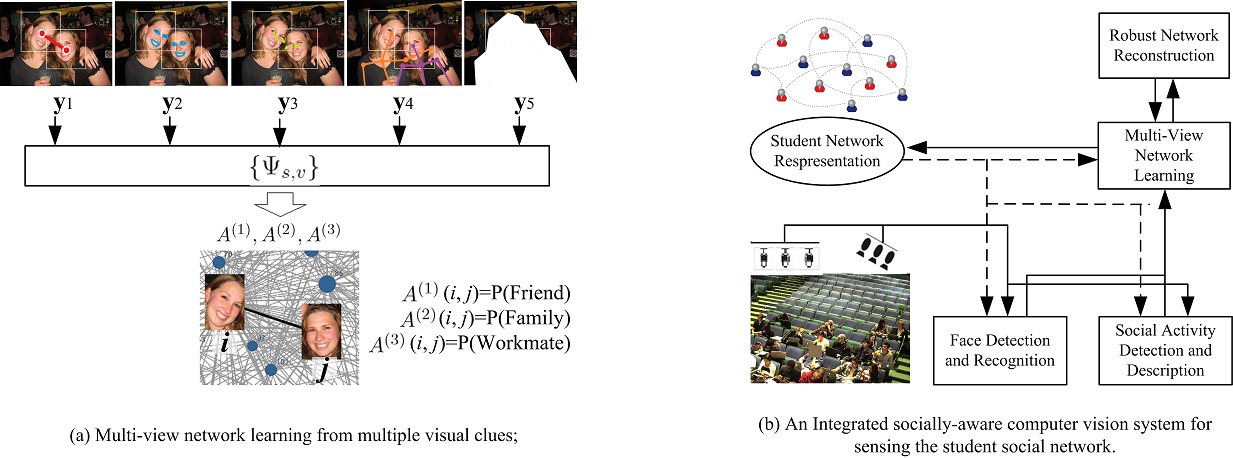
\includegraphics[width=\columnwidth]{featurelearn}
%\end{center}
%\vspace{-0.25in} \caption{\captionsize 
%Illustrations for the problem of multi-view network learning from multiple low-level visual clues and the framework of integrated socially-aware computer vision for understanding student netwrok. \label{fig:featurelearn}\afterfigspace}
%\end{figure}




%%%%%%%%%%%%%%%%%%%%%%%%%%%%%%%%%%%%%%%%%%%%%%%%%%%%%%%%%

%\subsubsection{Associating identities with image targets}
%\label{sec:assoc}

\boldstart{Associating identities with image targets}. To infer a social network from descriptors extracted from detected and tracked agents, we must first associate these vision-based descriptors with the identities of the tracked agents. While face recognition and identity recognition have progressed tremendously during the past decade (see Section~\ref{sec:background}), these systems will continue to suffer from uncertainty well into the future, especially when the input images and videos are low in quality. A key challenge we will address, therefore, is how to succeed in spite of this uncertainty. In doing so we will depart from most existing approaches in network reconstruction (e.g.,~\cite{}\todd{can you add any citations here?}), where even though additive or multiplicative noise might exist in the measured social affinities, these measurements are properly associated with the correct identities/nodes.

One simple approach we will explore is as follows. Suppose we have detected and tracked $L$, and that a face recognition system outputs for each a $K$-dimensional probability histogram $h_l(k)$ describing the likelihood of target $l$ being identity $k$. If facial recognition were perfect, each pair of  tracks would be used to produce one set of visual cues $\vy^s(i,j)$ linked the (certain) identities $i$ and $j$. In the presence of uncertainty, we can enumerate all possible $\prod_{l=0}^{L-1}(K-l)$  assignments, and then (conceptually) duplicate the video $\prod_{l=0}^{L-1}(K-l)$ times considering in each copy that the $L$ targets are assigned according to one of the possible assignments $\{k_1, k_2, \cdots, k_L\}, k_l\in\{1,2, \cdots, K\}$. This produces multiple outputs from each visual source---a descriptor of the form $\vy^s(k_i,k_j)$ for each of the $\prod_{l=0}^{L-1}(K-l)$ conceptual copies. 

The advantage of this approach is that it allows aggregating all of the information available from the recognition system, which we do by ``pooling'' the visual descriptors from all $\prod_{l=0}^{L-1}(K-l)$ copies. We will consider maximum-pooling approaches, $k_l^{*}=\max_{k}h_l(k)$, that select the most probable identity for target $l$ and use only the maximum assignment $\{k_1^{*}, k_2^{*}, \cdots, k_L^{*}\}$ to compute the social cues $\vy^s$ associated with identities $\{k_1^{*}, k_2^{*}, \cdots, k_L^{*}\}$. This strategy essentially assigns each target to a single (possibly incorrect) identity. We will also consider weighted average pooling, where every video copy corresponding to assignment $\{k_1, k_2, \cdots, k_L\}$ contributes to the social cues $\vy^s$ but with a confidence score proportional to the confidence of the recognition system, e.g., $\prod_{l=1}^{L}h_l(k_l)$. In this research, we will not just pursue good empirical results. We will also pursue tractable statistical models for identity uncertainty that can be characterized mathematically, with the goal of creating knowledge that can be more broadly applied to statistical signal processing on graphs and other relational data structures. 
\subsubsection{Noisy and incomplete network reconstruction}
\label{sec:reconstruct}

In many situations, images and videos from which we extract the multi-source cues are of low qualities, human beings are under significant pose variation, occlusion, and clutter, and most importantly, computer vision is imperfect and may frequently be incapable of yielding reliable outcomes for the network estimation to use. Consequently, the effects of invisible (missing) and noisy links, i.e., that an edge in the graph cannot be evaluated with a weighted affinity, will be particularly prevalent in a visually sensed social network. While this scenario is related to the traditional link prediction \cite{Goldberg,Liben-Nowell,TaskarWAK03} and receives preliminary treatment in network completion \cite{Clauset,Guimera,HannekeX09,KimL11}, we propose to explore better alternatives specific to the multi-view visually sensed network.

As a preliminary approach, we first re-represent the undirected weighted graph of $K$ nodes as $G$ describing the connections of $K$ members, where $G\triangleq\{A^{(v)}, Q^{(v)}\}, v=1,2,\cdots,V$, $A^{(v)}$ is the $K\times K$ affinity matrix for the $v$th view, and $Q^{(v)}$ is the $K\times K$ visibility matrix for that view. If $Q^{(v)}(i,j)=1$, then $A^{(v)}(i,j)$ is the weight describing the tie or closeness between node $i$ and node $j$ estimated from the $v$th view; otherwise if $Q^{(v)}(i,j)=0$ then $A^{(v)}(i,j)$ is a missing number indicating the lack of information of this link in this view. Our objective is to fill the missing links ($Q^{(v)}(i,j)=0$) with a proper weight for this partially observed multi-view network. 

%In the case that the views directly correspond to low-level visual cues, we may imagine that the ties between the pairs of members should not vary among different views due to different sensing modalities, and therefore there exist a unique community structure underlying all views. A primary objective in this case, is that how we may discover the community (clustering) effect from this partially observed multi-view network, together with filling the missing links with a proper weight. We refer to this primary task as network reconstruction.

The multi-view representation implies to exploit the mutual contexts provided from one view to another view. One may imagine that if the invisibles and gross errors are incoherent across views, visible and reliable affinities from other views will embed important information about this noisy view, and one may even find a `view-invariant' representation for the different views. To this end, we imagine that if each node $i$ in the graph can be uniquely identified with a point $\vx_i$ in an Euclidean space, then the distance between each pair of points $(i,j)$ in that space can be regarded as the `view-invariant' dissimilarity between the two nodes, and the view-specific affinity $A^{(v)}(i,j)$ may be derived from certain view-specific transform of the Euclidean distance. The question whether these conjectures can be successful now boils down to the question whether there exists a universal connection between Euclidean distances and arbitrary graph affinities.

The answer is YES. We have proved the following theorem, which implies that arbitrary graph affinities may always be analytically transformed into Euclidean distances between points. The proof of the theorem is based on Multi-Dimensional Scaling (MDS) \cite{CoxMDS}, and is omitted due to space limitation.

\vspace{5pt}
\textbf{Theorem}. \textit{If $A$ is symmetric affinity matrix with all zeros on the diagonal and positive numbers everywhere else, then there exists a constant $c$ such that $(\frac{1}{A(i,j)^2}+c)^{\frac{1}{2}}$ is the Euclidean distance between point $i$ (representing node $i$) and point $j$ (representing node $j$) in an Euclidean space, where $c\geq\lambda$, the smallest eigenvalue of $\Lambda=H\Gamma H$, $H=\mathbf{I}-\frac{\mathbf{1}\mathbf{1}^T}{K}$, and $\Gamma(i,j)=-\frac{1}{2A(i,j)^2}$.} 
\vspace{5pt}


The above theorem provides theoretical guarantee that each member (node) can be uniquely identified with a point in a Euclidean space, because now the Euclidean embedded nodes $\vx_i$'s and the generic social network representation $G$ are naturally related as
\begin{equation}\label{eq:embed}
(\vx_i-\vx_j)^{T}\Sigma^{(v)}(\vx_i-\vx_j)=\left(\frac{1}{A^{(v)}(i,j)^2}+c^{(v)}\right)^{\frac{1}{2}}+\epsilon^{(v)}_{ij}, \forall Q^{(v)}(i,j)=1,
\end{equation}
where $\Sigma^{(v)}$ is a symmetric semi-positive definite matrix specific to the $v$th view and $\epsilon$ is a residual. The technique that we adopt is new when compared to existing embedding ideas \cite{Hoff01latentspace,Hancocklatent}, multi-view networks \cite{AiroldiBFX08,Kim12}, and network completion \cite{Clauset,Guimera,HannekeX09,KimL11}, because it seamlessly unifies Eucliean embedding, multi-views, and missing data together, and more effectively exploits mutual contexts among view rather than other generic network constraints, which has not been attempted by existing social network research. In fact, any application-dependent network priors or regularizations are straightforward to be characterized through the embedded points $\vx_i$. 


%A unified community clustering effect, as the social network prior, may consequently  be modeled in the Euclidean space as well, for example, via
%\begin{equation}\label{eq:kmeans}
%Z=\arg\min_{D,\hat{Z}}\|X-D\hat{Z}\|^{2}_{2}, \textup{s.t.} \hat{Z}^{T}\mathbf{1}=\mathbf{1},
% \end{equation}
%where $X=[\vx_1,\vx_2,\cdots,\vx_K]$, each column of $D$ represents the center of a cluster, and $Z, \hat{Z}$ are a binary matrices by which we assign a node to a cluster among the communities of interest given by $D$. Upon learning the overall model incorporating the essential components in (\ref{eq:embed})(\ref{eq:kmeans}). It is straightforward to reconstruct the noisy and the missing affinities through transforms of Euclidean distances, and to investigate the underlying community structure invariant of views.

\subsubsection{Closing the loop}
\label{sec:closeloop}

A significant distinction of the proposed research on network reconstruction, is that it naturally collaborates with other modules in our framework and leverages our previous technical contribution: identity association (Section \ref{sec:assoc}) and network reconstruction (Section \ref{sec:reconstruct}), in fact, benefit from each other and constitute a close loop for improved social network estimation. Specifically, consider that if a less accurate face recognizer provides weak confidence about identities, and the error is propagated to low-level cues $\vy$. As a result, the estimated multi-view networks is noisy. By exploiting the `view-invariance' and reconstructing the affinities, we essentially get a de-noised version of the multi-view network. The enhanced or reduced ties between nodes conversely provide updated implication about the correct identity association for the two image targets, which may essentially be achieved via PI Zicker's previous contribution on joint face recognition using social contexts \cite{Stone2008,Stone2010} or their adapted versions. In other words, the proposed set of approaches in Section \ref{sec:vis2net} will essentially collaborate together.
% !TEX root = SocialVision2012.tex

\subsection{Datasets and Challenge Problems}
\label{sec:sys}

\begin{figure}[t!]
\begin{center}
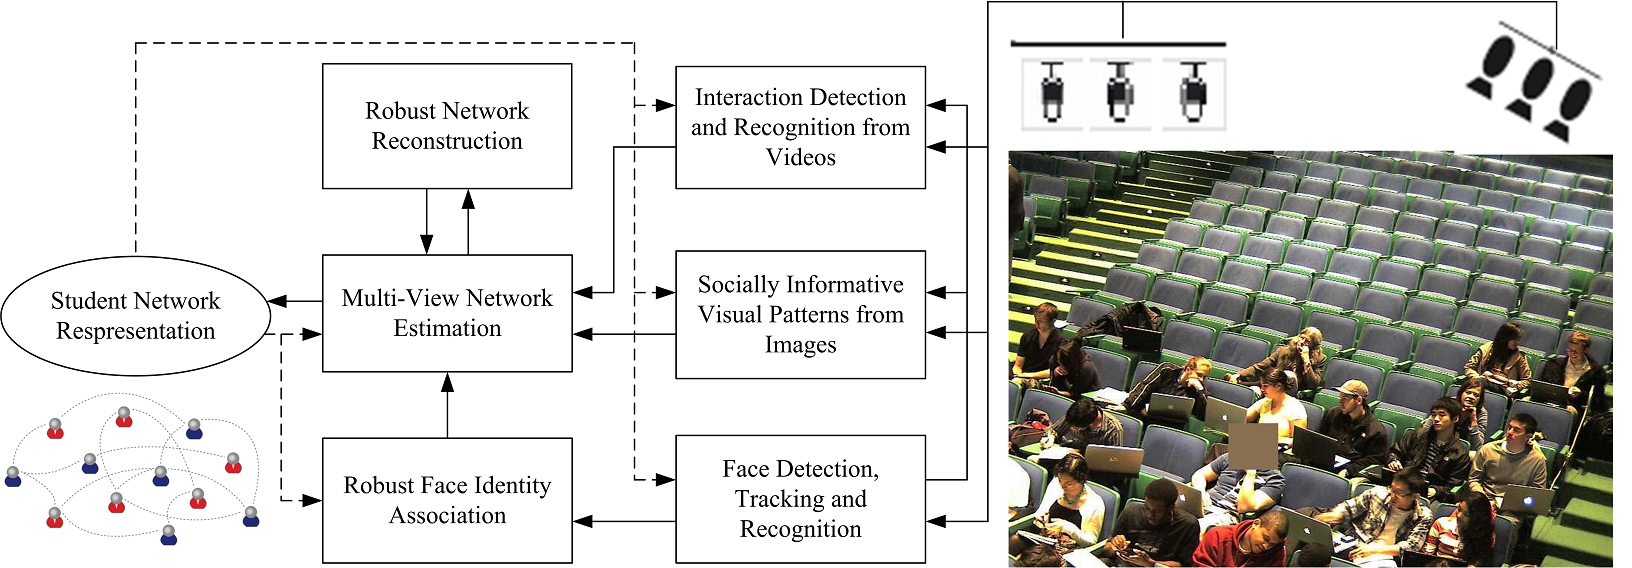
\includegraphics[width=\columnwidth]{prototype_1}
\end{center}
\vspace{-0.25in} \caption{\captionsize 
(a) The prototype hardware and software infrastructure for analyzing moderately constrained socialized human behaviors in an indoor environment for social network estimation at Harvard University; (b) Severely constrained UT Interaction dataset \cite{UTdata}; (c) Unconstrained New York Grand Central Station dataset \cite{WangMG09}.}\label{fig:prototype}\end{figure}

Our goal is to build a foundation for social analysis in diverse, unconstrained environments like that depicted in the bottom-right of Fig.~\ref{fig:prototype}(a). This is becoming well within reach thanks to the ready availability of networked camera arrays and advances in practical multi-view detection and tracking (e.g.,~\cite{EshelM10}). These unconstrained environments are fundamentally different from scenarios considered in existing benchmark datasets for interaction analysis (Fig.~\ref{fig:prototype}(b)(c)), where the interactions involve a pre-determined number of participants; take place in the absence of by-standers or social clutter; and/or are localized in time \emph{a priori}~\cite{UTdata,Choi:context,Choi:recogtrack,CRIM13}. Because of these  differences, evaluations on existing benchmarks fail to provide meaningful proxies for fundamental progress in large-scale social visual analysis.

As part of the proposed activity, we will create new datasets and challenge problems that make it possible to measure meaningful progress on social visual analysis, and at the same time, serve as a mechanism to engage the broader computer vision research community. To ensure that our benchmarks provide effective measures of progress, they will be annotated with ground-truth information about identities, interaction categories, and social relationships. We will create and use two distinct types of datasets. The first type will be based on video collections that are already being collected in large interactive classrooms at Harvard University. These datasets will be large (more than 350 camera-hours of video have been collected so far) and will enable evaluation of all aspects of the proposed research program, but because of the need for maintaining privacy of the observed subjects they will not be made directly available to non-collaborating research groups. The second type of datasets will supplement the first by being made publicly available. These will be smaller collections of annotated videos that contain interactions staged by informed actors, and they will simulate unconstrained environments by including long videos of large social gatherings. These will enable the evaluation of some aspects of the proposed research program (e.g., detecting interaction categories) and will be presented as ``challenge problems" for the broader computer vision research community.

\subsubsection{Harvard Interactive Classroom Datasets}
We will leverage video that is currently being collected by a six-camera array in a large interactive classroom at Harvard University. This system, which we call ``Lens to Learning'', has been developed over the past three years with funding by the NSF (IIS-0835338, 2009--2012) and the Harvard Initiative for Learning and Teaching (HILT)\footnote{\href{http://hilt.harvard.edu/2012-2013-awards}{http://hilt.harvard.edu/2012-2013-awards}} with the goal of understanding how students learn in interactive classrooms. The observed classroom is ``interactive'' in that students frequently engage in ad-hoc discussions. One commonly used technique is \emph{Peer Instruction}, which involves brief student discussions during the time traditionally devoted to lecture. Each discussion begins with a single ConcepTest---a question designed to elicit common student misconceptions [19,70]\cite{fix these references by copying the citations from the same sentence in the ALT proposal}. The students are given a moment to formulate and electronically submit their individual answer to the question posed, and then they are asked to form ad-hoc discussion groups to try to convince neighboring students of the correctness of their answers. After a few minutes of peer-to-peer discussion, students submit their possibly-revised answers, and this entire activity is usually followed by the instructor�s reinforcement of the main concept. Education research shows that both high and low ability students benefit from these discussions [24,36,80,83].\cite{fix these references by copying the citations from the same sentence in the ALT proposal}

The videos collected by Lens to Learning present an extraordinary opportunity for developing and evaluating large-scale social visual analysis. The observed classrooms---part of one is shown in Fig.~\ref{fig:prototype}(a), contain a hundred or more individuals engaged in ad-hoc interactions, and this creates a social environment that is fundamentally different from previous datasets (e.g., Fig.~\ref{fig:prototype}(b)(c)) in which interactions are  pre-localized in space or time. The utility of our interactive classrooms for social visual research stems not only from the number and diversity of people they contain, but from the nature of the interactions, the duration of our observations, and the non-visual sources of metadata available for validation. Individuals typically remain seated and forward-facing, and this simplifies detection and tracking, allowing us to focus our research on the higher-level challenges of detecting and recognizing social interactions. Also, for each course, videos are collected in every lecture over three-month semesters (about 200 camera-hours per course), enabling thorough evaluation of our methods for aggregating visual interaction data to infer social network information. This evaluation is made meaningful because of immense efforts being made by educational experts (funded by other sources and using techniques like those in [92]) to define a small number of semantically-meaningful interaction categories and painstakingly annotate occurrences of these interactions in the videos. This means, for example, that we can use the proposed techniques to discover and detect large numbers of interaction categories and then measure the degree to which some of them agree with the much smaller number that could be analyzed by human experts. Furthermore, in addition to video data, we have access to many non-visual sources of social network information (audio recordings from 48 omnidirectional boundary microphones mounted inconspicuously among the seats; educational outcomes; answers to ConcepTests; section assignments; gender; age; ethnicity; housing assignments, etc.) that allow some cross-validation of the social networks that we reconstruct from visual data.

To automatically analyze the videos collected by the Lens to Learning system, we have already developed a  suite of computer vision tools for ``pre-processing'' via face and body detection and tracking. This includes implementations of face detection and tracking, identity recognition, and head pose estimation, that together  provide large numbers of time-varying individual and pairwise descriptors ($\mathbf{f}_{m,t}$ and $\mathbf{g}_{m,m',t}$ in Section~\ref{sec:activity}) to be used as input to our methods. This dataset is affected by many sources of noise (false detections, missed detections, uncertain identities, uncertain pose) and is therefore a good proxy for many real-world environments. While this pre-processing suite provides a useful starting point for our research, we will continue to develop it during the award period to include richer descriptors such as histograms of flow and space-time interest points that capture elements of body pose and gesture. 

In conjunction with the Institutional Review Board at Harvard University, we have established a protocol in which classroom videos are recorded with consent from students and instructors, and then stored and analyzed on VPN-protected servers. More than 95\% of students also provide consent for their videos to appear in academic publications and presentations, allowing us to disseminate our research results through all of the regular academic channels. But since the classroom videos cannot be made directly available to research groups other than ours, we will promote reproducible research in three different ways. First, as described in the next section, we will create smaller parallel  datasets that are publicly-available and allow other research groups to evaluate algorithms for certain aspects of social visual analysis. Second, we will welcome interested research groups to collaborate with us to evaluate their algorithms on our classroom data by running their code on our VPN-protected servers. Third, whenever possible we will make use of advancing  technologies for privacy-preserving social science research---like those currently being developed by colleagues at Harvard University\footnote{\href{http://privacytools.seas.harvard.edu}{http://privacytools.seas.harvard.edu}}---to enable more direct sharing of classroom data for research purposes.

\subsubsection{Challenge problems}

An encouraging trend in computer vision over the last several years has been the increasing use of benchmark datasets for evaluating progress on particular tasks. Standardized datasets, such as the Middlebury Stereo Evaluation project~\cite{ScharsteinS02}, the PASCAL VOC Challenges~\cite{Everingham10}, the Berkeley Segmentation Database~\cite{MartinFTM01}, and the KTH database of individual actions~\cite{KTH}, have served as catalysts for progress on difficult problems because they create concrete targets that inspire new ideas and allow researchers to evaluate their systems by quantitatively demonstrating improvement. Currently, there are relatively few datasets available for problems related to social visual analysis, and those that do exist consider severely constrained environments that are not good proxies for the real world.

As part of the proposed activity, we will create new datasets and define challenge problems that engage the computer vision research community in our research agenda. \todd{Need more here -- details about a staged interaction dataset that we will create to evaluate interaction detection}

We will publish side-by-side comparisons of our performance on these public shared benchmarks and corresponding benchmarks derived from our  private classroom data. This is a strategy that PI Zickler has previously employed for research on private photo collections~\cite{PintoZickler2011}, and it means that any researcher who evaluates their algorithms on our (staged) public datasets can obtain an estimate of how well those same algorithms would perform in a  real classroom environment.


%With this established classroom observation system and these fundamental modules, we have successfully collected and processed a large-scale classroom behavior database consisting of 100 video clips in total. The students are seated in a regular lecture hall and are observed by a camera array with non-overlapping fields of view. The classroom is ``interactive'' because at various times throughout the lecture students are invited to engage in ad-hoc group discussions about problems provided by the instructor. The scale of our database is orders of magnitude larger than state-of-the-art computer vision datasets (e.g. those used in \cite{UTdata,Choi:context,Choi:recogtrack}), in the number of individuals (10-50 students per camera), the number of cameras (6), and the amount of time (100 minutes per camera, per recording, equaling over 3,000 minutes in total). Through a combination of face detection and tracking, we obtained noisy tracks for all students in each monocular video, upon which we developed descriptive modules that directly extract descriptiors such as head pose and body motion, we have also implemented a high-level module for behavior analysis based on similarity between two social groups, as depicted in Fig. \ref{fig:prototype}(b). In this module, the behavior of each individual is represented by a combination of the head pose and the motion of torso and arms (using the method of histogram of optical flows). The social behavior of a group is then represented by the configuration in space and time of the behaviors of its participants. With this social activity representation, the module detects a salient social activity from a new video and retrieves similar social activities from our established database. This functionality is illustrated in Fig. \ref{fig:prototype}(b), where our system has discovered a three-way conversation by identifying the participants of this conversation and the time span (several to tens of seconds) of this event. Based on the behavior representation for this space-time social interaction, the system searches the remainder of the database and retrieves a list of exemplars containing similar social behavior, ranked in the descending order of the similarities with the query. In this way, any manual annotations associated with the query video can be propagated to the top-ranking exemplars, and we are now taking this approach to propagate our manual annotations across the whole database. 








%At the current and initial stage of the effort to bring socialized semantics to computer vision, it can be usually the case that we do not have sufficient social contexts to help improving our target/face recognition, and we are not always specific about what are the meaningful social interactive activities that are most informative for social description. Conversely, we may neither know clearly about what exactly we should distill from images to fulfill a network learning task, nor have concrete knowledge about how the multiple views or overlapping community structures of a network will eventually turn out to be. However, we have argued at the beginning and demonstrated through the four proposed research problems the fact that the two aspects assist and benefit from each other, and an overall socially-aware visual analytical system is our ultimate goal. To this end, our final proposed research will include an attempt for a framework that eventually integrate social information and image understanding and allow them to learn and self-build themselves in an evolving and unsupervised manner.






% !TEX root =  SocialVision2012.tex
\vspace{-8pt}
\section{Broader Impacts}
\label{sec:impacts}
\vspace{-8pt}
A framework that enables social understanding from visual data is critical for computer vision systems to meet or exceed the human ability to understand the world from its images. While these ideas have received some attention from the research community, before now we have not had the resources to pursue it in any practical, real-world way. The accelerating development of computational infrastructure, the growth of digital video, and progress in detecting and tracking faces and people has finally made this research possible. 

The proposed  program will seize on this opportunity by concentrating our team's resources on the creation of a  framework for social visual analytics.  We will engage in its creation undergraduate and graduate students, the computer vision research community, and the broader public. These are critical steps toward a future in which machines can better understand and interact with their environments; and they will usher in radical changes to security, personal robotics, augmented reality, human-computer interfaces, security, and video summarization, to name a few.

Our research will also transform computational research in sociology, economics, and education, by providing researchers with access to social patterns that are difficult or impossible to detect with the naked eye. Traditionally, the analysis of interactions from video data has required immense effort by experts. A collections of videos must be viewed repeatedly before salient and meaningful interaction categories can be defined, and their occurrences in new videos must be painstakingly and redundantly coded by trained human observers (e.g.,~\cite{Scherr2009}). Our research will transform machine analyses in these disciplines by greatly simplifying the process of defining interaction categories, by automating the detection of instances of these interactions, and by automatically reconstructing social relationships from these detections. This will enable analyses in a much wider set of environments and over much longer periods of time.

The proposed research program will play an important role in education at both the undergraduate and graduate levels. The fundamental results of this research will be incorporated into the curricula of an existing computer vision class, enhancing senior undergraduate and graduate student education at the participating institution. Undergraduates at the junior and senior levels will be given opportunities for hands-on research experience, including summer research internships that may be funded by future NSF REU supplements. Finally, funding will be used to support two PhD, and these students will be an integral part of both research and educational endeavors in this project. They will participate in all stages, including the design of equipment and algorithms, and presentation of results at major conferences.

Our results will be broadly disseminated in three ways. First, they will be distributed by publications in refereed conferences and journals and by lectures at other institutions.  Second, datasets and source code will be posted online so that they can be easily adopted and extended (see attached Data Management Plan). Third, they will be shared through challenge problem workshops on social visual analytics, held in conjunction with the major  vision conferences, with the small amount of required funding provided by sponsorship agreements. The research team has an established track record in this type of outreach, with PI Zickler having organized tutorials in  vision and  graphics (ICCV 2007, SIGGRAPH 2008) as well as a workshops on computer vision (CRICV 2009, CRICV 2010, CPCV 2011)

\vspace{-8pt}
\section{Prior NSF Support}
\vspace{-10pt}
\boldstart{PI Todd Zickler} has been funded through a number of NSF awards to study computer vision. The most relevant are: ``Technological and Educational Foundations for Understanding and Improving Large-classroom Learning'' (IIS-0835338, 2009--2012, \$400,000), which supported the creation of the classroom observation system described in Section~\ref{sec:sys} and some analysis of this data for education purposes; and ``Computer Vision and Online Communities: A Symbiosis'' (HCC-0905243, 2009--2013, \$334,695) which supports research on the complementary problem of improving visual recognition by using a known social network as context. These awards have partially supported two PhD students and two post-doctoral fellows, and produced benchmark datasets for face recognition in personal photo collections~\cite{PintoZickler2011} and several notable publications~\cite{Stone2010,owens2011learning,LiZickler2012,xiong2012pixels}.

\boldstart{PI Ruonan Li} has not previously been supported by the NSF.



\clearpage
\bibliographystyle{plain} \bibliography{social_Li,vision_Li,egbib,graph_prop,kapoor,NSF_HCC,transfer,xtrabib,zicklerpubs}


\end{document}

